  %------------------------------------------------------------------------------
% Beginning of journal.tex
%------------------------------------------------------------------------------
%
% AMS-LaTeX version 2 sample file for journals, based on amsart.cls.
%
%        ***     DO NOT USE THIS FILE AS A STARTER.      ***
%        ***  USE THE JOURNAL-SPECIFIC *.TEMPLATE FILE.  ***
%
% Replace amsart by the documentclass for the target journal, e.g., tran-l.
%
\documentclass[12pt, reqno]{amsart}

%     If your article includes graphics, uncomment this command.



\usepackage{graphicx}

\usepackage{amssymb,amsmath,amsthm}
\usepackage{esint}
%\usepackage{mathrsfs}
%\usepackage{comment}
%\usepackage{bbm,dsfont,bm}
%\usepackage{cite}
\usepackage{color}
\usepackage[left=1.5cm, right=1.5cm, top=1.8cm, bottom=1.8cm]{geometry}

\theoremstyle{definition}
%\usepackage{libertine}
%\usepackage{tgtermes}DO NOT ADD!!!!!

\newtheorem{assumption}[equation]{Assumption}
\newtheorem{theorem}[equation]{Theorem}
\newtheorem{lemma}[equation]{Lemma}
\newtheorem{corollary}[equation]{Corollary}
\newtheorem{conjecture}[equation]{Conjecture}
\newtheorem{definition}[equation]{Definition}
\newtheorem{example}[equation]{Example}
\newtheorem{remark}[equation]{Remark}
\newtheorem{proposition}[equation]{Proposition}


\usepackage{graphicx}
\newcommand{\bfu}{{\bf u}}
\def\BBN {{\mathbb N}}
\def\BBZ {{\mathbb Z}}
\def\BBQ {{\mathbb Q}}
\def\BBR {{\mathbb R}}
\def\BBC {{\mathbb C}}
%\newcommand{\abs}[1]{|{#1}|}
\newcommand{\norm}[1]{{\left \Vert{#1}\right \Vert}}

 
%\usepackage[margin=1in]{geometry} 
\usepackage{amsmath,amsthm,amssymb,enumerate, fancyhdr}
\usepackage[english]{babel}
%\usepackage[square,sort,comma,numbers]{natbib}
\usepackage[backref=page]{hyperref}

\usepackage{thmtools}
\renewcommand\qedsymbol{$\blacksquare$}

\newcommand{\seb}[1]{{\color{blue}#1}}
\newcommand{\claudiu}[1]{{\color{magenta}#1}}
\newcommand{\Mindrila}{{M\^{i}ndril\u{a}}}
\newcommand{\curl}{{\mathrm{curl}}}
\newcommand{\setR}{\mathbb{R}}
\newcommand{\N}{\mathbb{N}}
\newcommand{\divergence}{\mathrm{div}}
\newtheorem*{theorem*}{Theorem}

\newcommand{\bfq}{\mathbf{q}}
\newcommand{\weakto}{\rightharpoonup}

\newcommand{\Arm}{\mathrm{A}}
\newcommand{\Brm}{\mathrm{B}}
\newcommand{\Crm}{\mathrm{C}}
\newcommand{\Drm}{\mathrm{D}}
\newcommand{\Erm}{\mathrm{E}}
\newcommand{\Frm}{\mathrm{F}}
\newcommand{\Grm}{\mathrm{G}}
\newcommand{\Hrm}{\mathrm{H}}
\newcommand{\Irm}{\mathrm{I}}
\newcommand{\Jrm}{\mathrm{J}}
\newcommand{\Krm}{\mathrm{K}}
\newcommand{\Lrm}{\mathrm{L}}
\newcommand{\Mrm}{\mathrm{M}}
\newcommand{\Nrm}{\mathrm{N}}
\newcommand{\Orm}{\mathrm{O}}
\newcommand{\Prm}{\mathrm{P}}
\newcommand{\Qrm}{\mathrm{Q}}
\newcommand{\Rrm}{\mathrm{R}}
\newcommand{\Srm}{\mathrm{S}}
\newcommand{\Trm}{\mathrm{T}}
\newcommand{\Urm}{\mathrm{U}}
\newcommand{\Vrm}{\mathrm{V}}
\newcommand{\Wrm}{\mathrm{W}}
\newcommand{\Xrm}{\mathrm{X}}
\newcommand{\Yrm}{\mathrm{Y}}
\newcommand{\Zrm}{\mathrm{Z}}

\newcommand{\Acal}{\mathcal{A}}
\newcommand{\Bcal}{\mathcal{B}}
\newcommand{\Ccal}{\mathcal{C}}
\newcommand{\Dcal}{\mathcal{D}}
\newcommand{\Ecal}{\mathcal{E}}
\newcommand{\Fcal}{\mathcal{F}}
\newcommand{\Gcal}{\mathcal{G}}
\newcommand{\Hcal}{\mathcal{H}}
\newcommand{\Ical}{\mathcal{I}}
\newcommand{\Jcal}{\mathcal{J}}
\newcommand{\Kcal}{\mathcal{K}}
\newcommand{\Lcal}{\mathcal{L}}
\newcommand{\Mcal}{\mathcal{M}}
\newcommand{\Ncal}{\mathcal{N}}
\newcommand{\Ocal}{\mathcal{O}}
\newcommand{\Pcal}{\mathcal{P}}
\newcommand{\Qcal}{Q_L }
\newcommand{\Rcal}{\mathcal{R}}
\newcommand{\Scal}{\mathcal{S}}
\newcommand{\Tcal}{\mathcal{T}}
\newcommand{\Ucal}{\mathcal{U}}
\newcommand{\Vcal}{\mathcal{V}}
\newcommand{\Wcal}{\mathcal{W}}
\newcommand{\Xcal}{\mathcal{X}}
\newcommand{\Ycal}{\mathcal{Y}}
\newcommand{\Zcal}{\mathcal{Z}}

\newcommand{\Afrak}{\mathfrak{A}}
\newcommand{\Bfrak}{\mathfrak{B}}
\newcommand{\Cfrak}{\mathfrak{C}}
\newcommand{\Dfrak}{\mathfrak{D}}
\newcommand{\Efrak}{\mathfrak{E}}
\newcommand{\Ffrak}{\mathfrak{F}}
\newcommand{\Gfrak}{\mathfrak{G}}
\newcommand{\Hfrak}{\mathfrak{H}}
\newcommand{\Ifrak}{\mathfrak{I}}
\newcommand{\Jfrak}{\mathfrak{J}}
\newcommand{\Kfrak}{\mathfrak{K}}
\newcommand{\Lfrak}{\mathfrak{L}}
\newcommand{\Mfrak}{\mathfrak{M}}
\newcommand{\Nfrak}{\mathfrak{N}}
\newcommand{\Ofrak}{\mathfrak{O}}
\newcommand{\Pfrak}{\mathfrak{P}}
\newcommand{\Qfrak}{\mathfrak{Q}}
\newcommand{\Rfrak}{\mathfrak{R}}
\newcommand{\Sfrak}{\mathfrak{S}}
\newcommand{\Tfrak}{\mathfrak{T}}
\newcommand{\Ufrak}{\mathfrak{U}}
\newcommand{\Vfrak}{\mathfrak{V}}
\newcommand{\Wfrak}{\mathfrak{W}}
\newcommand{\Xfrak}{\mathfrak{X}}
\newcommand{\Yfrak}{\mathfrak{Y}}
\newcommand{\Zfrak}{\mathfrak{Z}}

\newcommand{\afrak}{\mathfrak{a}}
\newcommand{\bfrak}{\mathfrak{b}}
\newcommand{\cfrak}{\mathfrak{c}}
\newcommand{\dfrak}{\mathfrak{d}}
\newcommand{\efrak}{\mathfrak{e}}
\newcommand{\ffrak}{\mathfrak{f}}
\newcommand{\gfrak}{\mathfrak{g}}
\newcommand{\hfrak}{\mathfrak{h}}
\newcommand{\ifrak}{\mathfrak{i}}
\newcommand{\jfrak}{\mathfrak{j}}
\newcommand{\kfrak}{\mathfrak{k}}
\newcommand{\lfrak}{\mathfrak{l}}
\newcommand{\mfrak}{\mathfrak{m}}
\newcommand{\nfrak}{\mathfrak{n}}
\newcommand{\ofrak}{\mathfrak{o}}
\newcommand{\pfrak}{\mathfrak{p}}
\newcommand{\qfrak}{\mathfrak{q}}
\newcommand{\rfrak}{\mathfrak{r}}
\newcommand{\sfrak}{\mathfrak{s}}
\newcommand{\tfrak}{\mathfrak{t}}
\newcommand{\ufrak}{\mathfrak{u}}
\newcommand{\vfrak}{\mathfrak{v}}
\newcommand{\wfrak}{\mathfrak{v}}
\newcommand{\xfrak}{\mathfrak{x}}
\newcommand{\yfrak}{\mathfrak{y}}
\newcommand{\zfrak}{\mathfrak{z}}

\newcommand{\Asf}{\mathsf{A}}
\newcommand{\Bsf}{\mathsf{B}}
\newcommand{\Csf}{\mathsf{C}}
\newcommand{\Dsf}{\mathsf{D}}
\newcommand{\Esf}{\mathsf{E}}
\newcommand{\Fsf}{\mathsf{F}}
\newcommand{\Gsf}{\mathsf{G}}
\newcommand{\Hsf}{\mathsf{H}}
\newcommand{\Isf}{\mathsf{I}}
\newcommand{\Jsf}{\mathsf{J}}
\newcommand{\Ksf}{\mathsf{K}}
\newcommand{\Lsf}{\mathsf{L}}
\newcommand{\Msf}{\mathsf{M}}
\newcommand{\Nsf}{\mathsf{N}}
\newcommand{\Osf}{\mathsf{O}}
\newcommand{\Psf}{\mathsf{P}}
\newcommand{\Qsf}{\mathsf{Q}}
\newcommand{\Rsf}{\mathsf{R}}
\newcommand{\Ssf}{\mathsf{S}}
\newcommand{\Tsf}{\mathsf{T}}
\newcommand{\Usf}{\mathsf{U}}
\newcommand{\Vsf}{\mathsf{V}}
\newcommand{\Wsf}{\mathsf{W}}
\newcommand{\Xsf}{\mathsf{X}}
\newcommand{\Ysf}{\mathsf{Y}}
\newcommand{\Zsf}{\mathsf{Z}}

\newcommand{\Abf}{\mathbf{A}}
\newcommand{\Bbf}{\mathbf{B}}
\newcommand{\Cbf}{\mathbf{C}}
\newcommand{\Dbf}{\mathbf{D}}
\newcommand{\Ebf}{\mathbf{E}}
\newcommand{\Fbf}{\mathbf{F}}
\newcommand{\Gbf}{\mathbf{G}}
\newcommand{\Hbf}{\mathbf{H}}
\newcommand{\Ibf}{\mathbf{I}}
\newcommand{\Jbf}{\mathbf{J}}
\newcommand{\Kbf}{\mathbf{K}}
\newcommand{\Lbf}{\mathbf{L}}
\newcommand{\Mbf}{\mathbf{M}}
\newcommand{\Nbf}{\mathbf{N}}
\newcommand{\Obf}{\mathbf{O}}
\newcommand{\Pbf}{\mathbf{P}}
\newcommand{\Qbf}{\mathbf{Q}}
\newcommand{\Rbf}{\mathbf{R}}
\newcommand{\Sbf}{\mathbf{S}}
\newcommand{\Tbf}{\mathbf{T}}
\newcommand{\Ubf}{\mathbf{U}}
\newcommand{\Vbf}{\mathbf{V}}
\newcommand{\Wbf}{\mathbf{W}}
\newcommand{\Xbf}{\mathbf{X}}
\newcommand{\Ybf}{\mathbf{Y}}
\newcommand{\Zbf}{\mathbf{Z}}

\newcommand{\Abb}{\mathbb{A}}
\renewcommand{\Bbb}{\mathbb{B}}
\newcommand{\Cbb}{\mathbb{C}}
\newcommand{\Dbb}{\mathbb{D}}
\newcommand{\Ebb}{\mathbb{E}}
\newcommand{\Fbb}{\mathbb{F}}
\newcommand{\Gbb}{\mathbb{G}}
\newcommand{\Hbb}{\mathbb{H}}
\newcommand{\Ibb}{\mathbb{I}}
\newcommand{\Jbb}{\mathbb{J}}
\newcommand{\Kbb}{\mathbb{K}}
\newcommand{\Lbb}{\mathbb{L}}
\newcommand{\Mbb}{\mathbb{M}}
\newcommand{\Nbb}{\mathbb{N}}
\newcommand{\Obb}{\mathbb{O}}
\newcommand{\Pbb}{\mathbb{P}}
\newcommand{\Qbb}{\mathbb{Q}}
\newcommand{\Rbb}{\mathbb{R}}
\newcommand{\Sbb}{\mathbb{S}}
\newcommand{\Tbb}{\mathbb{T}}
\newcommand{\Ubb}{\mathbb{U}}
\newcommand{\Vbb}{\mathbb{V}}
\newcommand{\Wbb}{\mathbb{W}}
\newcommand{\Xbb}{\mathbb{X}}
\newcommand{\Ybb}{\mathbb{Y}}
\newcommand{\Zbb}{\mathbb{Z}}

%\DeclareMathOperator{\esssup}{ess\,sup}
\DeclareMathOperator{\id}{id}
\DeclareMathOperator{\clos}{cl}
\DeclareMathOperator{\co}{co}
\newcommand{\cocl}{\mathop{\cl{\co}}}
\DeclareMathOperator{\interior}{int}
\DeclareMathOperator{\dom}{dom}
\DeclareMathOperator{\img}{img}
\DeclareMathOperator{\diam}{diam}
\DeclareMathOperator{\graph}{graph}
\DeclareMathOperator*{\wlim}{w-lim}
\DeclareMathOperator*{\wslim}{w*-lim}
\DeclareMathOperator*{\Splim}{\ensuremath{\Scal^\prime}-lim}
\DeclareMathOperator{\limmod}{lim}
\DeclareMathOperator{\liminfmod}{lim\,inf}
\DeclareMathOperator{\limsupmod}{lim\,sup}
\DeclareMathOperator{\infmod}{inf}
\DeclareMathOperator{\supmod}{sup}
\DeclareMathOperator{\diverg}{div}
\DeclareMathOperator{\Diverg}{Div}
%\DeclareMathOperator{\curl}{curl}
\DeclareMathOperator{\dist}{dist}
\DeclareMathOperator{\rank}{rank}
\DeclareMathOperator{\tr}{tr}
\DeclareMathOperator{\spn}{span}
\DeclareMathOperator{\ran}{ran}
\DeclareMathOperator{\supp}{supp}
\DeclareMathOperator{\cof}{cof}
\DeclareMathOperator{\diag}{diag}
\DeclareMathOperator{\Ad}{Ad}
\DeclareMathOperator{\ad}{ad}
\DeclareMathOperator{\dev}{dev}
\DeclareMathOperator{\proj}{proj}
%\DeclareMathOperator{\sgn}{sgn}
\DeclareMathOperator{\Argmin}{Argmin}
\DeclareMathOperator{\Sgn}{Sgn}

\newcommand{\ee}{\mathrm{e}}
\newcommand{\ii}{\mathrm{i}}
\newcommand{\set}[2]{\left\{\, #1 \ \ \textup{\textbf{:}}\ \ #2 \,\right\}}
\newcommand{\setn}[2]{\{\, #1 \ \ \textup{\textbf{:}}\ \ #2 \,\}}
\newcommand{\setb}[2]{\bigl\{\, #1 \ \ \textup{\textbf{:}}\ \ #2 \,\bigr\}}
\newcommand{\setB}[2]{\Bigl\{\, #1 \ \ \textup{\textbf{:}}\ \ #2 \,\Bigr\}}
\newcommand{\setBB}[2]{\biggl\{\, #1 \ \ \textup{\textbf{:}}\ \ #2 \,\biggr\}}
\newcommand{\setBBB}[2]{\Biggl\{\, #1 \ \ \textup{\textbf{:}}\ \ #2 \,\Biggr\}}
%\newcommand{\norm}[1]{\|#1\|}
\newcommand{\normlr}[1]{\left\|#1\right\|}
\newcommand{\normn}[1]{\|#1\|}
\newcommand{\normb}[1]{\bigl\|#1\bigr\|}
\newcommand{\normB}[1]{\Bigl\|#1\Bigr\|}
\newcommand{\normBB}[1]{\biggl\|#1\biggr\|}
\newcommand{\normBBB}[1]{\Biggl\|#1\Biggr\|}
\newcommand{\abs}[1]{|#1|}
\newcommand{\abslr}[1]{\left|#1\right|}
\newcommand{\absn}[1]{|#1|}
\newcommand{\absb}[1]{\bigl|#1\bigr|}
\newcommand{\absB}[1]{\Bigl|#1\Bigr|}
\newcommand{\absBB}[1]{\biggl|#1\biggr|}
\newcommand{\absBBB}[1]{\Biggl|#1\Biggr|}
\newcommand{\floor}[1]{\lfloor #1 \rfloor}
\newcommand{\floorlr}[1]{\left\lfloor #1\right\rfloor}
\newcommand{\floorn}[1]{\lfloor #1\rfloor}
\newcommand{\floorb}[1]{\bigl\lfloor #1\bigr\rfloor}
\newcommand{\floorB}[1]{\Bigl\lfloor #1\Bigr\rfloor}
\newcommand{\floorBB}[1]{\biggl\lfloor #1\biggr\rfloor}
\newcommand{\floorBBB}[1]{\Biggl\lfloor #1\Biggr\rfloor}
\newcommand{\spr}[1]{( #1 )}
\newcommand{\sprlr}[1]{\left( #1 left)}
\newcommand{\sprn}[1]{( #1 )}
\newcommand{\sprb}[1]{\bigl( #1 \bigr)}
\newcommand{\sprB}[1]{\Bigl( #1 \Bigr)}
\newcommand{\sprBB}[1]{\biggl( #1 \biggr)}
\newcommand{\sprBBB}[1]{\Biggl( #1 \Biggr)}
\newcommand{\dpr}[1]{\langle #1 \rangle}	
\newcommand{\dprlr}[1]{\left\langle #1 \right\rangle}
\newcommand{\dprn}[1]{\langle #1 \rangle}
\newcommand{\dprb}[1]{\bigl\langle #1 \bigr\rangle}
\newcommand{\dprB}[1]{\Bigl\langle #1 \Bigr\rangle}
\newcommand{\dprBB}[1]{\biggl\langle #1 \biggr\rangle}
\newcommand{\dprBBB}[1]{\Biggl\langle #1 \Biggr\rangle}
\newcommand{\ddpr}[1]{\langle\!\langle #1 \rangle\!\rangle}
\newcommand{\ddprlr}[1]{\left\langle\!\left\langle #1 \right\rangle\!\right\rangle}
\newcommand{\ddprn}[1]{\langle\!\langle #1 \rangle\!\rangle}
\newcommand{\ddprb}[1]{\bigl\langle\hspace{-2.5pt}\bigl\langle #1 \bigr\rangle\hspace{-2.5pt}\bigr\rangle}
\newcommand{\ddprB}[1]{\Bigl\langle\!\!\Bigl\langle #1 \Bigr\rangle\!\!\Bigr\rangle}
\newcommand{\ddprBB}[1]{\biggl\langle\!\!\biggl\langle #1 \biggr\rangle\!\!\biggr\rangle}
\newcommand{\ddprBBB}[1]{\Biggl\langle\!\!\Biggl\langle #1 \Biggr\rangle\!\!\Biggr\rangle}
\newcommand{\cl}[1]{\overline{#1}}
\newcommand{\di}{\mathrm{d}}
\newcommand{\dd}{\;\mathrm{d}}
\newcommand{\DD}{\mathrm{D}}
%\newcommand{\N}{\mathbb{N}}
%\newcommand{\R}{\mathbb{R}}
%\newcommand{\C}{\mathbb{C}}
%\newcommand{\Q}{\mathbb{Q}}
%\newcommand{\Z}{\mathbbZ}
\newcommand{\loc}{\mathrm{loc}}
\newcommand{\sym}{\mathrm{sym}}
\newcommand{\skw}{\mathrm{skew}}
\newcommand{\per}{\mathrm{per}}
\newcommand{\start}{\mathrm{start}}
\newcommand{\ex}{\times}
\newcommand{\sing}{\mathrm{sing}}
\newcommand{\ONE}{\mathbbm{1}}
\newcommand{\tolong}{\longrightarrow}
\newcommand{\toto}{\rightrightarrows}
\newcommand{\toweak}{\rightharpoonup}
\newcommand{\toweakstar}{\overset{*}\rightharpoonup}
\newcommand{\towsloc}{\overset{*}\rightharpoondown_\loc}
\newcommand{\tosquig}{\rightsquigarrow}
\newcommand{\toup}{\uparrow}
\newcommand{\todown}{\downarrow}

\newcommand{\embed}{\hookrightarrow}
\newcommand{\cembed}{\overset{c}{\embed}}
\newcommand{\conv}{\star}
\newcommand{\BigO}{\mathrm{\textup{O}}}
\newcommand{\SmallO}{\mathrm{\textup{o}}}
\newcommand{\sbullet}{\begin{picture}(1,1)(-0.5,-2.5)\circle*{2}\end{picture}}
\newcommand{\frarg}{\,\sbullet\,}
\newcommand{\BV}{\mathrm{BV}}
\newcommand{\BD}{\mathrm{BD}}
\newcommand{\BMO}{\mathrm{BMO}}
\newcommand{\LD}{\mathrm{LD}}
\newcommand{\GY}{\mathbf{GY}}
\newcommand{\BDY}{\mathbf{BDY}}
\newcommand{\MCF}{\mathbf{MCF}}
\newcommand{\WF}{\mathrm{WF}}
\newcommand{\toS}{\overset{s}{\to}}
\newcommand{\toB}{\overset{b}{\to}}
\newcommand{\toLOne}{\overset{\Lrm^1}{\to}}
\newcommand{\toY}{\overset{\mathrm{Y}}{\to}}
\newcommand{\toYloc}{\overset{\mathrm{Y}_\loc}{\tolong}}
\newcommand{\toSp}{\overset{\Scal'}{\to}}
\newcommand{\toMCF}{\overset{\mathrm{MCF}}{\tolong}}
\newcommand{\eps}{\epsilon}
\newcommand{\lrangle}[1]{\langle #1 \rangle}	

\DeclareMathOperator{\Lie}{Lie}
\DeclareMathOperator{\Var}{Var}
\DeclareMathOperator{\Exp}{Exp}
\DeclareMathOperator{\Li}{Li}
\DeclareMathOperator{\Ls}{Ls}
\DeclareMathOperator{\Lt}{Lt}
\DeclareMathOperator{\Diss}{Diss}

\newcommand{\term}[1]{\textbf{#1}}
\newcommand{\person}[1]{\textsc{#1}}
\newcommand{\assumptionhead}[1]{\emph{#1}}
\newcommand{\proofstep}[1]{\emph{#1}}
\newcommand{\GL}{\mathrm{GL}}
\newcommand{\SO}{\mathrm{SO}}
\newcommand{\SL}{\mathrm{SL}}
\newcommand{\bfX}{\mathbf{X}}


%SEBASTIAN STUFF
%\usepackage[frak,operator]{paper_diening}
\newcommand{\meantmp}[2]{#1\langle{#2}#1\rangle}
\newcommand{\mean}[1]{\meantmp{}{#1}}
\newcommand{\bigmean}[1]{\meantmp{\big}{#1}}
\newcommand{\Bigmean}[1]{\meantmp{\Big}{#1}}
\newcommand{\biggmean}[1]{\meantmp{\bigg}{#1}}
\newcommand{\Biggmean}[1]{\meantmp{\Bigg}{#1}}
\providecommand{\skptmp}[3]{{\ensuremath{#1\langle {#2}, {#3} #1\rangle}}}
\providecommand{\skp}[2]{\skptmp{}{#1}{#2}}
\newcommand{\nablasym}{{\nabla_s}}

\DeclareMathOperator{\divg}{div}
\DeclareMathOperator{\bog}{Bog}
\DeclareMathOperator{\ext}{Ext}
\DeclareMathOperator{\test}{\Fcal_{\eta}}
\DeclareMathOperator{\testn}{Test_{\eta^{\varepsilon_n}}}
\DeclareMathOperator{\testd}{\Fcal_{\delta}}
%\DeclareMathOperator{\sym}{sym}
\DeclareMathOperator{\cor}{\Kcal_{\eta}}
\newcommand{\bn}{{\nu}}
\newcommand{\bfp}{\mathbf{p}}
\newcommand{\Bogovskij}{{Bogovski\u{\i}}{}}
\newcommand{\bfPsi}{\mathbf{\Psi}}
\newcommand{\bfPhi}{\mathbf{\Phi}}
%END SEBASTIAN STUFF

\numberwithin{equation}{section}

%    Absolute value notation
%\newcommand{\abs}[1]{\lvert#1\rvert}

%    Blank box placeholder for figures (to avoid requiring any
%    particular graphics capabilities for printing this document).
\newcommand{\blankbox}[2]{%
  \parbox{\columnwidth}{\centering
%    Set fboxsep to 0 so that the actual size of the box will match the
%    given measurements more closely.
    \setlength{\fboxsep}{0pt}%
    \fbox{\raisebox{0pt}[#2]{\hspace{#1}}}%
  }%
}
\usepackage{graphicx}
\usepackage{tikz}


\begin{document}


\title[Time-periodic weak solutions for FSI]{Time-periodic weak solutions for the interaction of an incompressible fluid with a linear Koiter type shell under dynamic pressure boundary conditions}
%Newtonian fluid interacting with a Koiter type shell under no-slip boundary conditions.}

%    Information for first author
\author{Claudiu M\^{i}ndril\u{a}}
%    Address of record for the research reported here
\address{Department of Analysis, Faculty of Mathematics and Physics, Charles University,
Sokolovsk\'{a} 83, 18675, Prague, Czech Republic }
\email{mindrila@karlin.mff.cuni.cz}
%    \thanks will become a 1st page footnote.
%\thanks{The first author was supported in part by NSF Grant \#000000.}

%    Information for second author
\author{Sebastian Schwarzacher}
\address{Department of Analysis, Faculty of Mathematics and Physics, Charles University,
Sokolovsk\'{a} 83, 18675, Prague, Czech Republic }
\email{schwarz@karlin.mff.cuni.cz}
%\thanks{Support information for the second author.}

%    General info
%\subjclass[2000]{Primary 54C40, 14E20; Secondary 46E25, 20C20}

\date{\today}

%\dedicatory{This paper is dedicated to our advisors.}

%\keywords{Mathematics!}

\begin{abstract}
In many occurrences of fluid-structure interaction time-periodic motions are observed. We consider the interaction between a fluid driven by the three dimensional Navier-Stokes equation and a two dimensional linearized elastic Koiter shell situated at the boundary. The fluid-domain is a part of the solution and as such changing in time periodically. On a steady part of the boundary we allow for the physically relevant case of dynamic pressure boundary values, prominent to model inflow/outflow. We provide the existence of at least one weak time-periodic solution for given periodic external forces that are not to large. For that we introduce new approximation techniques and a-priori estimates.
\end{abstract}

%\noindent\textsc{MSC (2010):35Q35 (primary); 35Q30, 35J60, 35J70, 35J75.} 



\maketitle
\noindent\textsc{Keywords:} Navier-Stokes equations,  Periodic solutions, Fluid-structure interaction, Koiter shell



\section{Introduction}

Periodic motions are often observed when fluids and solids are interacting. This phenomenon ranges from large motions as the rotation of wind-wheels to flutter. It includes important applications such as heart-beat driven blood flow through vessels or oscillations of bridge decks~\cite{pironneau1994optimal,Quarteroni2000,FSIforBIO,C21} and important benchmarks from numerics as in~\cite{turek.s.hron.j:numerical}. In this work some answers to the related relevant question {\em under what conditions time-periodic motions may occur mathematically} are given.

The interaction between fluids and solids is an intensive domain of research. There is a vast list of results in many scientific areas. While most results are in the applied sciences including applied mathematics more and more pure mathematical results are being  proved. For an overview on the analytical results and related applications for the set-up considered here, that is the setting of a moving shell constituting a part of the boundary of the fluid with which it is in interaction, we refer to the excellent survey \cite{C21} and the references therein.
As can be seen there, the focus in the study of {\em weak solutions} is on the {\em existence of solutions for the Cauchy problem}, that is solutions whose initial values are given. We mention here the pioneering results obtained by Grandmont et. al.~\cite{Gr05,Gr08} for the case of a plate, and by Lengeler and R\r{u}{\v{z}}i{\v{c}}ka in \cite{LR14} for the case of a linear shell. Further extensions were obtained in \cite{MS22}  where the Cauchy problem for the \emph{nonlinear Koiter energy} was proved, along some additional regularity estimates. For the initial value problem further extension are compressible or heat-conducting fluids
\cite{BreSch18,breit-schwarz-fourier} and the {\em constructive} existence results by means of Arbitrary-Lagrangian-Eulerian methods obtained by Muha and Cani{\'c} in \cite{muha-canic-arma-13,muha-canic-noslip}. There dynamic pressure conditions where investigated that are prominent for blood-vessel simulations.  See also \cite{KamSchSpe23} where deformations in all coordinate directions were considered.

In comparison to the Cauchy problem, much less research was devoted to the time-periodic problem. The first results in this regime was obtained by the authors of this paper~\cite{our-paper}. Please see there other references for previous results on time-periodic solutions for strong solutions, fixed fluid-domain or most significantly rigid body motions~\cite{galdi2006existence,galdi2020viscous}.

In this paper we continue the study on {\em time-periodic solutions for fluid-structure interactions involving shells}. For the fluid we consider the {\em unsteady three dimensional Navier-Stokes equation} while the shell is moving in a prescribed direction along a potentially {\em curved} reference geometry. We consider a linearized Koiter energy type, the one rigorously justified in \cite{Ci05}. Hence the evolution of the solid is {\em hyperbolic and linear}. The shell is situated on a part of the fluid-boundary which hence is time-changing. On a steady part of the fluid-boundary we consider pressure boundary values. Our main result is Theorem~\ref{thm:main}, where the existence of coupled time-periodic weak solutions to such interactions (namely~\eqref{eqn:system}) is shown for all time-periodic forces, which size is not larger then a constant essentially depending on the curvature of the reference geometry in relation to the stiffness of the elastic shell. See Figure~\ref{figure} for the typical geometric set up. The current work is an extension of~\cite{our-paper}.
\begin{itemize}
\item In~\cite{our-paper} the solid was considered to be a flat plate. Accordingly the motion of the shell was restricted to a fixed coordinate axis. In the present paper curved reference configurations are allowed and the motion of the shell is then along the non-trivial normal vector-bundle. In dependence of the principle curvatures of the reference configurations further restrictions on the size of the admissible forces where unavoidable. However the dependencies are quantified in a controlled manner and vanish in the flat plate case.
\item There is a difference in the boundary conditions. While in~\cite{our-paper} everywhere no-slip boundary conditions where considered, in the present paper on a part of the boundary pressure boundary conditions are considered. What we show is that this quite prominent setting for applications~\cite{C21} seems to be very appropriate to expect the appearance of time-periodic motions, see Remark~\ref{rem:noslip}. 
\end{itemize}
The crucial technical reason for why there are much more existence results for the Cauchy problem in relation to time-periodic solutions lies in the fact that the so-called {\em energy estimates} are very different.
Indeed, as in the time periodic setting initial and end value cancel the {\em energy estimates} are here {\em significantly weaker}. In case the structure is not viscous, this means essentially no estimate for it by the {\em energy inequality} that is not coming from the fluid. Hence, a second {\em regularity estimate} for the structure is unavoidable. This was already realized in \cite{our-paper}. The technical innovation in the present paper however lies directly in the construction of the solution. Already the Galerkin basis (commonly the first step to find a solution) is constructed along the {\em extra regularity estimates} that are unavoidable in the time-periodic setting. 
This construction allows to perform all necessary estimates in the very first approximation step. 

We believe this innovation to be rather suitable for further applications. 
A few are summarized in several remarks that follow Theorem~\ref{thm:main}, where also limitations of the approach are discussed. This includes the treatment of further boundary conditions (see Remark~\ref{rem:boundary} and Remark~\ref{rem:noslip}).





\subsection{The model}
Let $I=[0,T]$ be a time-interval. 
We define $\Omega\subset \mathbb{R}^3$ the  reference configuration for the fluid domain, which is assumed to be open, bounded, connected  with  a $C^3$-boundary. We shall denote the tangential unit vectors by $\tau_1,\tau_2$ and the  outer normal by $\nu$. 
The boundary of $\Omega$ consists of three parts. First, $M$ the moving part of the boundary which is determined by the motion of the shell,  which is assumed to be clamped at its endpoints. This part of the boundary is naturally parametrized by the deformation of the structure. 
Second, $\Gamma_p$ the inflow and outflow part of the boundary. 
It is a steady component of $\partial \Omega$.% and for simplicity we assume that the normal vector field to $\Gamma_p$  is  $\nu= (0,0, \pm 1)$. 
Finally the Dirichlet part $\Gamma_D$ of the boundary on which we assume homogenuous no-slip boundary conditions $\mathbf{u}=\mathbf{0}$. 
Note that this part needs not  to be large, but we assume that it has a non-negative (surface) measure.\footnote{An inflow in terms of a non-zero Dirichlet boundary value would be meaningful. The present method seems to be suitable to allow for inhomogenuous periodic boundary values as well. Restrictions on the regularity or size of the boundary values should be expected.} Both Dirichlet and inflow/outflow boundary parts are steady in time, while the moving part of the boundary changes {\em via the solid deformation that is assumed to move in direction of the fixed direction of the outer normal of the domain}. In particular, this model reduction implies that the velocity in tangential direction of the fluid is assumed to be zero along the shell. This is a much used model reductions see~\cite{Ci05}. Indeed, the theory of weak-solution for shells that are modelled to move freely in all coordinate directions has only recently been initiated~\cite{KamSchSpe23}. 
%The situation is depicted in the figure~\ref{figure}.
\begin{figure}\label{figure}
\caption{The domain $\Omega_{\eta(t)}$}
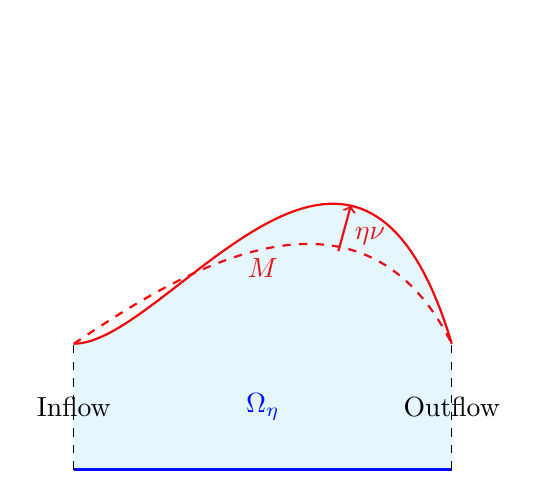
\begin{tikzpicture}[scale=0.8]
\draw[thick,red]   (8, 2) .. controls (9.5, 2) and (12.5, 7) .. (14, 2);
\draw[thick,dashed,red]   (8, 2) .. controls (9.5, 3) and (12.5, 5) .. (14, 2);
%\draw[thick,dashed]   (8.5, 0.5) .. controls (9.5, 1) and (12.5, 3) .. (13.5, 0.5);
%\draw[thick,dashed]   (7, 3.5) .. controls (9.5, 5) and (12.5, 8) .. (15, 3.5);
%\draw[thick,dashed]   (5.65, 0.2) .. controls (6.2,2.7) .. (7, 3.5);
%\draw[thick,dashed]   (14, 0)--(15,3.5);
%\draw[thick,dashed](8,0)--(14,0)--(14,2)--(8,2)--(8,0);
\draw[very thick, blue](8,0)--(14,0);
\path node at (11,1) {\textcolor{blue}{$\Omega_\eta$}};
\path node at (11,3.2) {\textcolor{red}{\bf $M$}};
\draw[->,thick, red] (12.2,3.47)--(12.4,4.2);
%\draw[<->,thick] (10.1,1.3)--(8.5,4.4);
\path node at (12.7,3.7) {\textcolor{red}{\bf $\eta\nu$}};
%\path node at (10,2.5) {\textcolor{black}{\bf $-L\nu$}};
%\path node at (9.3,3.7) {\textcolor{black}{\bf $L\nu$}};
\fill[color=cyan,opacity=.1]  (8, 2) .. controls (9.5, 2) and (12.5, 7) .. (14, 2) -- (14,0) -- (8,0) -- (8,2);
%\draw[thick,black]   (8, 1.2) .. controls (6.7, 1) and (4,0) .. (7,0);
%\draw[thick](7,0)--(12,0);
%\draw[thick,black]   (8, 1.2) .. controls (12.5, 3) .. (14, 1.2);
\draw[dashed](8, 0) -- (8, 2);
\draw[dashed](14, 0) -- (14, 2);
%\draw[thick,black]   (14, 1.2) .. controls (13.5, 0.5) .. (12, 0);
%\path node at (7,0.5) {\textcolor{black}{ supp$\psi^L$}};
\path node at (8,1) {\textcolor{black}{Inflow}};
\path node at (14,1) {\textcolor{black}{Outflow}};
%\path node at (12,1.3) {\textcolor{black}{ $Q_L$}};
%\path node at (11,5) {\textcolor{black}{ $Q^L$}};
\end{tikzpicture}
\end{figure}

Concerning the moving part $M$, we assume that it is parametrized by  a map $\phi$ and an open set $\omega \subset  \mathbb{R}^{2}$ via 
\begin{equation}
M=\phi\left(\omega\right),\ \phi\in C^{4}\left(\omega;\mathbb{R}^{3}\right),\ \phi\ \text{injective}
\end{equation}
This enables us to define the tangent vectors $\partial_{1} \phi (y)$ and $\partial_{2} \phi (y)$ at each point of $\phi(y)$, $y \in \omega$ and the unit normal vector field as 
\begin{equation}
\nu : \omega \mapsto S^{1}, \  \nu\left(y\right):=\frac{\partial_{1}\phi\left(y\right)\times\partial_{2}\phi\left(y\right)}{\left|\partial_{1}\phi\left(y\right)\times\partial_{2}\phi\left(y\right)\right|}, \quad y\in \omega.
\end{equation}
On the moving part we attach an \emph{elastic shell} which moves only in normal direction and 
 whose displacement field  is  $\eta \nu $ 
 where 
 \[
\eta : \omega \mapsto \mathbb{R}.
\]
Then $\eta$ is extended by zero to $\mathbb{R}^{2}$, which corresponds to a clamped shell.
Thus, the mapping
\begin{equation}\label{eqn:phi-eta-t}
\phi_{\eta}:\omega\mapsto\phi_{\eta}\left(\omega\right),\quad\phi_{\eta}:x\mapsto\phi\left(x\right)+\eta\left(t,x\right)\nu_{\phi\left(x\right)}
\end{equation} 
is a parametrization of  the boundary $\partial\Omega_\eta$
 of the moving domain  $\Omega_\eta$,  which can be thought to be  the interior of the surface bounded by  $\partial \Omega_\eta$.
Here $\chi_M$ denotes the characteristic function on $M$. Observe that $\phi_{\eta}$
is a homeomorphism and even a $C^{k}$ diffeomorphism if $\eta \in C^{k}_0(\omega)$ and $\phi^{-1}\in C^{k}(M)$ for $k \in \mathbb{N}$.
We now  introduce  the  \emph{deformed time-space cylinders} for times $t\in I$ and deformations $\eta : I \times \omega \mapsto \mathbb{R}$ 
 throughout \[
I\times\Omega_{\eta}:=\bigcup_{t\in I}\left\{ t\right\} \times\Omega_{\eta\left(t\right)}.
\]

The mapping $\phi_{\eta(t)}$ from \eqref{eqn:phi-eta-t}   extends  to a homomorphism 
\begin{equation}\label{eqn:psi-eta-t}
\psi_{\eta\left(t\right)}:\Omega\mapsto\Omega_{\eta\left(t\right)},\quad t\in I
\end{equation}
and defines a diffeomorphism (whose regularity depends on $\eta$).
Note that, in particular, self-penetrations are excluded.





\subsubsection*{The Koiter elastic energy}\label{subsection:Koiter}
Following \cite[Theorem 4.2.1]{Ci05}, we introduce the  
% \emph{linearized change of metric tensor} by 
%\begin{equation}\label{eqn:tensor-metric}
%\mathbb{G}_{ij}\left(\eta\right):=\left[\partial_{i}\phi_{\eta}\cdot\partial_{j}\phi_{\eta}-\partial_{i}\phi\cdot\partial_{j}\phi\right]^{lin},\quad i,j=1,2.
%\end{equation}
%
%We consider the \emph{normal direction to the deformed surface}  $\nu_{\eta}$ 
%\begin{equation}
%\nu_{\eta}:=\partial_{1}\phi_{\eta}\times\partial_{2}\phi_{\eta}.
%\end{equation}
%More explicitly, it takes the form 
%\[
%\begin{aligned}
%\nu_{\eta}= & \left(\partial_{1}\phi\times\partial_{2}\right)\phi+\left(\partial_{1}\phi\times\nu_{\phi}\right)\partial_{2}\eta+\left(\partial_{1}\phi\times\partial_{2}\right)\nu_{\phi}\eta+\\
% & +\left(\nu_{\phi}\times\partial_{2}\phi\partial_{1}\right)\eta+\left(\nu_{\phi}\times\partial_{2}\nu_{\phi}\right)\left(\partial_{1}\eta\right)\eta+\left(\partial_{1}\nu_{\phi}\times\partial_{2}\phi\right)\eta\\
% & +\left(\partial_{1}\nu_{\phi}\times\nu_{\phi}\right)\partial_{2}\eta+\left(\partial_{1}\nu_{\phi}\times\partial_{2}\nu_{\phi}\right)\eta^{2}
%\end{aligned}
%\]
%The \emph{linearized change of curvature tensor} is then defined as
%\begin{equation}\label{eqn:tensor-curvature}
%\mathbb{R}_{ij}^{\sharp}:=\left[\frac{\partial_{ij}\phi_{\eta}\cdot\nu_{\eta}}{\left|\partial_{1}\phi\times\partial_{2}\phi\right|}-\partial_{ij}\phi\cdot\nu\right]^{\text{lin}},\quad i,j=1,2.
%\end{equation}
%
%All-in-all,  if  $h$ denotes the thickness of the shell,  then the 
\emph{linearized Koiter energy} for $h$ the thickness of the plate $\eta$, as $\mathbb{G}(\eta)$ the linearised metric tensor and $\mathbb{R}_{ij}^{\sharp}$ as the linearised curvature tensor:
\begin{equation}\label{eqn:Koiter-energy}
K\left(\eta\right):=\sum_{i,j,m,l=1}^{2}\frac{h}{2}\int_{\omega}\mathbb{A}^{ij, ml}\mathbb{G}_{ml}\left(\eta\right)\mathbb{G}_{ij}\left(\eta\right)dA+\frac{h^{3}}{6}\int_{\omega}\mathbb{A}^{ij, ml}\mathbb{R}^{\sharp}_{ml}\left(\eta\right)\mathbb{R}^{\sharp}_{ij}\left(\eta\right)dA.
\end{equation}
Here $\mathbb{A}$ is a fourth-order tensor known as \emph{the elasticity (or stiffness) tensor} defined through
\begin{equation}\label{eqn:lame}
\mathbb{A}^{ij,ml}=\frac{4\lambda \mu}{\lambda+2\mu}a^{ij}a^{ml}+4\mu (a^{im}a^{jl}+a^{il}a^{jm})
\end{equation}
 and $\lambda,  \mu$ are the Lam\'{e} coefficients and $a^{ij}$ is the contravariant metric tensor associated to $M$.
In \cite[Theorem 4.4.2]{Ci05} it is shown that, in fact, that the $L^2$ gradient of $K$ takes the form 
\[
K^{\prime}\left(\eta\right)=m\Delta^{2}\eta+B\eta.
\]
where $m>0$ is a constant depending on the elastic material and $B$ a second order differential operator.
It is also proved (in the same reference \cite{Ci05}) that the Koiter energy is $H^2$-coercive, that is there exists a positive constant $c_0>0$ for which 
\begin{equation}\label{eqn:c0-coercivity}
K\left(\eta\right)\ge c_{0}\left\Vert \eta\right\Vert _{H^{2}\left(\omega\right)}^{2}\quad\text{ for all }\eta\in H_{0}^{2}\left(\omega\right)
.\end{equation}
\subsubsection*{The equations}
Suppose now that at each time $t$ the domain $\Omega_{\eta(t)}$ is filled with an \emph{incompressible fluid}, whose velocity is $\mathbf{u}$ and pressure $p$ and fulfills the Navier-Stokes system. We consider here the  so-called \emph{dynamic pressure condition} $\frac{1}{2}\left|\mathbf{u}\right|^{2}+p=P$ where $P:I\times \Gamma_p\mapsto\mathbb{R}$ is a prescribed, time-periodic function. Other types of inflow/outflow boundary conditions could be treated by the methodology developed here (see Remark~\ref{rem:boundary}). 

Therefore the fluid equations  take the form
\begin{equation}\label{eqn:fluid}
\begin{cases}
\rho_f(\partial_{t}\mathbf{u}+\left(\mathbf{u}\cdot\nabla\right)\mathbf{u})=\text{\text{div}\ensuremath{\mathbb{T}}+\ensuremath{\mathbf{f}} } & \text{in}\ I\times\Omega_{\eta}\\
\text{div}\mathbf{u}=0 & \text{in}\ I\times\Omega_{\eta}\\
\rho_f\frac{\left|\mathbf{u}\right|^{2}}{2}+p=P& \text{on}\ I\times\Gamma_{p}\\
u\cdot\tau_{i}=0 & \text{on}\ I\times\Gamma_{p}\text{ for }i\in\{1,2\}.\\
\mathbf{u}=\mathbf{0} & \text{on}\ I\times\Gamma_{D}\\
\mathbf{u}\circ\phi_{\eta}=\left(\partial_{t}\eta\right)\nu & \text{on}\ I\times\omega\\
\mathbf{u}\left(0,\cdot\right)=\mathbf{u}\left(T,\cdot\right) & \text{in}\ \left\{ 0\right\} \times\Omega_{\eta\left(0\right)}
\end{cases}
\end{equation}

Here $\mathbb{T}$ is the usual \emph{Cauchy stress tensor}
 \begin{equation}\label{eqn:Cauchy-stress}
\mathbb{T}\left(\mathbf{u},p\right):=\sigma\cdot D\left(\mathbf{u}\right)-p\mathbb{I}_{3},\quad D\left(\mathbf{u}\right):=\frac{1}{2}\left(\nabla\mathbf{u}+\left(\nabla\mathbf{u}\right)^{T}\right)
\end{equation}
and $\sigma$  the fluid viscosity. 

Concerning now the shell displacement $\eta$, it solves   the wave-type equation
\begin{equation}\label{eqn:shell}
\begin{cases}
\rho_{S}h\partial_{tt}\eta+K^{\prime}\left(\eta\right)=g+\mathbf{F}\cdot\nu & \text{in}\ I\times\omega\\
\eta=\left|\nabla\eta\right|=0 & \text{on}\ I\times\partial\omega\\
\eta\left(0,\cdot\right)=\eta\left(T,\cdot\right) & \text{in}\ \omega
\end{cases}
\end{equation}
where $\rho_{S}>0$ is the density of the reference-shell. Here
$K^{\prime}(\eta)$ denotes the $L^{2}$ gradient of the functional $K(\eta)$ from \eqref{eqn:Koiter-energy} and therefore
\[
K\left(\eta,\xi\right):=\langle K'(\eta),\xi\rangle = m\int_\omega\nabla^2\eta\cdot \nabla^2\xi\, dA+ \langle B\eta,\xi\rangle\text{ for all }\eta,\xi\in H_{0}^{2}\left(\omega\right).
\]
Further, $\mathbf{F}$ is the force exerted by the fluid on the boundary of the domain and is  defined as
\begin{equation}\label{eqn:force-fluid-shell-normal}
\mathbf{F}\left(t,\cdot\right):=-\mathbb{T}\left(\mathbf{u},p\right)\nu_{\eta\left(t\right)}\circ\phi_{\eta\left(t\right)}\left|\det \nabla\phi_{\eta\left(t\right)}\right|.
\end{equation}
In the following we shall take for simplicity
\[
\sigma=\rho_f=\rho_S h=1.
\]
Let us now write the coupled system formed by \eqref{eqn:fluid} and \eqref{eqn:shell} to obtain the \emph{fluid-structure interaction problem} which consists in the following system
\begin{equation}\label{eqn:system}
\begin{cases}
\partial_{t}\mathbf{u}+\left(\mathbf{u}\cdot\nabla\right)\mathbf{u}=\text{\text{div}\ensuremath{\mathbb{T}}+\ensuremath{\mathbf{f}} } & \text{in}\ I\times\Omega_{\eta}\\
\text{div}\mathbf{u}=0 & \text{in}\ I\times\Omega_{\eta}\\
\frac{\left|\mathbf{u}\right|^{2}}{2}+p=P\left(t\right) & \text{on}\ I\times\Gamma_{p}\\
\mathbf{u}\cdot{\bf \tau}_{i}=0 & \text{on}\ I\times\Gamma_{p}\text{ for }i\in\{1,2\}\\
\mathbf{u}=\mathbf{0} & \text{on}\ I\times\Gamma_{L}\\
\mathbf{u}\circ\phi_{\eta}=\left(\partial_{t}\eta\right)\nu & \text{on}\ I\times\omega\\
\mathbf{u}\left(0,\cdot\right)=\mathbf{u}\left(T,\cdot\right) & \text{in}\ \left\{ 0\right\} \times\Omega_{\eta\left(0\right)}\\
\partial_{tt}\eta-K^{\prime}\left(\eta\right)=g+{\bf F}\cdot\nu & \text{in}\ I\times\omega\\
\eta\left(0,\cdot\right)=\eta\left(T,\cdot\right),\partial_{t}\eta\left(0,\cdot\right)=\partial_{t}\eta\left(T,\cdot\right) & \text{in}\ \omega\\
\left|\eta\right|=\left|\nabla\eta\right|=0 & \text{on}\ I\times\partial\omega.
\end{cases}
\end{equation}
\subsection{Main results}
Our main result has a quantitative dependence on how curved the reference geometry is. For that we introduce $\kappa_1(\bfp)$ and $\kappa_2(\bfp)$ as the two principle curvatures of $M$ at the point $\bfp$. Moreover we define
\[
\kappa:=\max_{\bfp\in M}\abs{\kappa_1(\bfp)}+\abs{\kappa_2(\bfp)}
\]
 as the maximal principal curvature of $M$. This is precisely the point where degeneration of the shell may happen most easily.

\begin{theorem}\label{thm:main}
Let $\Omega$ be a given reference domain with properties described as above. Then there exists a constant $\tilde{C}$ depending on $\Gamma_p,\Gamma_D,\kappa_1,\kappa_2,L,\abs{M}$ and $c_0$ such that if
$\left(\mathbf{f},g,P\right)\in L_{\text{per}}^{2}\left(I;L^2(\mathbb{R}^{3})\right)\times L_{\text{per}}^{2}\left(I;L^2(\omega)\right)\times L_{\text{per}}^{2}\left(I;L^2(\Gamma_p)\right)$ satisfies
\begin{equation}
\left\Vert \mathbf{f}\right\Vert _{L_{t}^{2}L_{x}^{2}}+\left\Vert g\right\Vert _{L_{t}^{2}L_{x}^{2}}+\left\Vert P\right\Vert _{L_{t}^{2}L_{x}^{2}}\le\tilde{C}
\end{equation}
then there exists at least one weak time-periodic solution $\left(\mathbf{u},\eta\right)$ as it is defined in Definition~\ref{def:weak-soln}. 
Furthermore, it enjoys the \emph{diffusion estimate}
\begin{align*}
\frac{1}{2}\int_{0}^{T}\int_{\Omega_{\eta\left(t\right)}}\left|\nabla\mathbf{u}\right|^{2}\,dx\leq\int_{0}^{T}\int_{\Omega_{\eta\left(t\right)}}\mathbf{f}\cdot{\bf u}\,dxdt+\int_{\omega}g\partial_{t}\eta\,dAdt+\int_{\Gamma_{p}}P{\bf u}\cdot\nu\,dAdt
\end{align*}
and the {\em additional regularity estimate}
\begin{equation}\label{eqn:main-energy-estimate}
\sup_{t\in I}E\left(t\right)+\left\Vert \mathbf{u}\right\Vert _{L_{t}^{2}W_{x}^{1,2}}^{2}\leq C,
\end{equation}
with $C$ depending on $\tilde{C}$, $\Gamma_p,\Gamma_D,\kappa_1,\kappa_2,L,\abs{M},c_0$ and $T$,
where we denote here and in the rest of the paper
\begin{equation}
    E\left(t\right):=\frac{1}{2}\int_{\Omega_{\eta\left(t\right)}}\left|\mathbf{u}\right|^{2}dx+\frac{1}{2}\int_{\omega}\left|\partial_{t}\eta\right|^{2}dA+K\left(\eta\left(t,\cdot\right)\right),\quad t\in I.
\end{equation}
\end{theorem}
\begin{remark}[On the size of $\tilde{C}$ and C] The constant $C$ is made precise in Proposition~\ref{prop:formal-decoupled-estimates} and depends linearly and quadratically on $\tilde{C}$.
We made quite an effort to make the dependence of $\tilde{C}$ on the reference geometry, the time interval and the Lam\'e constants precise. See again Proposition~\ref{prop:formal-decoupled-estimates} for the precise dependencies.

Important is that the constant $\tilde{C}$ that appears in Theorem~\ref{thm:main} has not to be small. The size is reduced first to ensure a-priori that a self-intersection is excluded and second to compensate for the curved reference geometry. Large forces are admissible if the Lam\'{e} coefficients are large (in comparison to their thickness), which resembled the case of a stiff thick solid. Indeed, for $c_0\to \infty$, we find $\tilde{C}\to \infty$. Moreover, the estimates in \cite{our-paper} are recovered as by letting $\kappa_1,\kappa_2\to 0$ in Proposition~\ref{prop:Solenoidal-extension-o}.
\end{remark}
\begin{remark}[Case $\Gamma_p=0$]
\label{rem:noslip}
In case no inflow or outflow is present, the mean-value of the pressure is determined by the shell. Hence the mean-value of the pressure is bound to depend on the Koiter energy. It is yet an open problem, how to derive an a-priori estimate in that case. An exception is the case, when $M$ is flat. This case was treated in \cite{our-paper}.
\end{remark}
\begin{remark}
\label{rem:boundary}
The boundary  condition $\frac{1}{2}\left|{\bf u}\right|^{2}+p=P_{\text{in/out }}$ representing the prescribed inflow/outflow contributes to the relatively simple weak formulation~\eqref{eqn:weak-form}.  Another alternative would have been to provide a Dirichlet inflow $\bf{u}=u_{D} \ \text{on} \ \Gamma_{\text{in}}$ and a so called "do-nothing" boundary condition which, actually, would consist in imposing $\mathbb{T}\nu=\frac{1}{2}\left|{\bf u}\right|^{2}\nu\ \text{on}\ \Gamma_{\text{out}}$, as it was rigorously justified by Bathory and Stefanelli in \cite{BaSt21}.
\end{remark}
%\begin{remark}
%\label{rem:nonnew}
% Due to the construction of the Galerkin approximation, it seems that the case of non-Newtonian fluids of $p$-type with $p \ge 2$ can be covered. This means that instead of the term $\Delta \mathbf{u}$, we consider the term $\Delta_{p}=\text{div}\left(\left|\nabla\mathbf{u}\right|^{p-2}\left|\nabla\mathbf{u}\right|\right)$. See \cite{Lengeler-p-fluid} for further details.
% \end{remark}
    Let us observe that our methodology also provides a proof of the following result. To our best knowledge, it was not considered in the literature. Compare with \cite[Theorem 3.5]{LR14}. %The proof is actually slightly simplified and  follows the same lines as of Theorem~\ref{thm:main}.
    \begin{theorem}
    \label{thm:cauchy}
        Let
        \[
\left(\mathbf{f},g,P\right)\in L_{\text{loc}}^{1}\left(\left[0,\infty\right);L_{\text{loc}}^{2}\left(\mathbb{R}^{3}\right)\right)\times L_{\text{loc}}^{1}\left(\left[0,\infty\right);L_{\text{loc}}^{2}\left(\omega\right)\right)\times L_{\text{loc}}^{2}\left(\left[0,\infty\right)\right)
        \]
 and let the initial-data 
 \[
\left(\mathbf{u}_{0},\eta_{0},\eta_{1}\right)\in L^{2}\left(\Omega_{\eta\left(0\right)}\right)\times H_{0}^{2}\left(\omega\right)\times L^{2}\left(\omega\right)
 \]
 be such that $\text{div}\mathbf{u}_{0}=0$ and $\text{tr}_{\eta_{0}}\mathbf{u}_{0}=\eta_{1}\nu$. Then, there exists a time $0<T^{*}\le \infty$ such that the corresponding initial-value problem admits a weak solution satisfying the usual energy inequality. The time $T^*<\infty$ only in case of topological changes of the boundary.
    \end{theorem}




\subsection{Mathematical strategy}
\label{sec:math}
Our approach towards the existence of a solution is the following: we decouple the problem by prescribing a time-periodic deformation $\delta$ 
and we prove that a time-periodic weak solution exists, by proving the time-periodicity and the relevant estimates at the Galerkin level already.
Then, in a second step, we perform a set-valued fixed-point $\delta \mapsto \eta$ to recover the coupling.

The strategy brings some novelty.
We modify the divergence-free extension operator introduced in \cite{MS22}, such that it enables us to create \emph{coupled} test functions of the form $\left(\mathcal{F}_{\delta}\left(\xi\right),\xi\right)$. It is also used in the construction of a Galerkin basis and in the proof of the $L^{2}$ compactness~\cite{breit-schwarz-fourier}.
In particular, the well chosen basis allows to gather al necessary information on the Galerkin level already. This menas here the non-standard a-priori estimates, the coupling between the PDE and the geometry and the time-periodicity. The method of using a suitable Galerkin basis seems to have some potential for future results in this area.
% It was this step which could not be  performed in \cite{LR14} (and neither in \cite{our-paper}). 
 





\subsection{Overview of the paper}
In Section~\ref{sec:prelim} we introduce the moving domains, the divergence-free extension operator $\mathcal{F}_{\delta}$ and introduce the definition of the time-periodic weak solution.
 
Section~\ref{sec:decoupled-problem} is dedicated to establish the key estimate, contained in Proposition~\ref{prop:formal-decoupled-estimates}. This means introducing the necessary estimates, the construction of according suitable decoupled approximations, the recovery of a time-periodic coupled solution via a fixed point argument and a limit passage.
The paper ends with Section~\ref{sec:Proof-main-thm} where we perform the proof of Theorem~\ref{thm:main} and Theorem~\ref{thm:cauchy}.

\section{Preliminaries}\label{sec:prelim}

\subsection{Function spaces on variable domains}\label{subsection:function-spaces}
For admisible domains $\Omega_{\eta}$ we introduce the Lebesgue and Sobolev spaces adapted to the moving domains $\Omega_{\eta}$ are defined as follows: for $1 \le p, \ q \le \infty$ we have
\begin{equation}
\begin{aligned}L^{p}\left(I;L^{q}\left(\Omega_{\eta}\right)\right):= & \left\{ \mathbf{v}\in L^{1}\left(I\times\Omega_{\eta}\right):\mathbf{v}\left(t,\cdot\right)\in L^{q}\left(\Omega_{\eta\left(t\right)}\right)\ \text{for a .e.}\ t\in I,\right.\\
 & \left\Vert \mathbf{v}\left(t,\cdot\right)\right\Vert _{L^{q}\left(\Omega_{\eta\left(t\right)}\right)}\in L^{p}\left(I\right)\left.\right\} \\
L^{p}\left(I;W^{1,q}\left(\Omega_{\eta}\right)\right):= & \left\{ \mathbf{v}\in L^{1}\left(I\times\Omega_{\eta}\right):\mathbf{v}\left(t,\cdot\right)\in W^{1,q}\left(\Omega_{\eta\left(t\right)}\right)\ \text{for a .e.}\ t\in I,\right.\\
 & \left\Vert \mathbf{v}\left(t,\cdot\right)\right\Vert _{L^{q}\left(\Omega_{\eta\left(t\right)}\right)}\in L^{p}\left(I\right)\left.\right\} 
\end{aligned}
\end{equation}
One can now introduce the corresponding \emph{time-periodic} spaces of functions $L_{\text{per}}^{p}\left(I;L^{q}\left(\Omega_{\eta}\right)\right)$ and resp. $L_{\text{per}}^{p}\left(I;W^{1,q}\left(\Omega_{\eta}\right)\right)$ obtained by taking the closure of the set $\left\{ \varphi\in C^{\infty}\left(I\times\mathbb{R}^{3}\right):\varphi\left(0,\cdot\right)=\varphi\left(T,\cdot\right)\right\} $ in the respective norms.

Then, given a time-periodic moving domain $\Omega_{\delta}$ determined by a displacement   $\delta\in C^{3}\left(\omega\right)$ with $\left\Vert \delta\right\Vert _{L_{t,x}^{\infty}}<L$ 
we can introduce the \emph{space of solutions} $V_{S}^{\delta}$  by
\begin{equation}
\begin{aligned}V_{S}^{\delta}:= & \left\{ \left(\mathbf{u},\eta\right):\mathbf{u}\in L_{\text{per}}^{2}\left(I;H_{\text{div}}^{1}\left(\Omega_{\delta}\right)\right)\times L_{\text{per}}^{\infty}\left(I;L^{2}\left(\Omega_{\delta}\right)\right),\right.\\
 & \eta\in L_{\text{per}}^{\infty}\left(I;H_{0}^{2}\left(\omega\right)\right)\cap W_{\text{per}}^{1,\infty}\left(I;L^{2}\left(\omega\right)\right),\mathbf{u}=0\text{ on }\Gamma_{D},\\
 & \mathbf{u}\cdot\tau_{1}=\mathbf{u}\cdot\tau_{2}=0\text{ on }\Gamma_{p},\mathbf{u}\circ\phi_{\delta}=\partial_{t}\eta\nu\text{ on }\omega\left.\right\} 
\end{aligned}
\end{equation}
and the corresponding \emph{space  of test-functions} $V_{T}^{\delta}$ by
\begin{equation}
\begin{aligned}V_{T}^{\delta}:= & \left\{ \left(\mathbf{q},\xi\right):\mathbf{q}\in W_{\text{per}}^{1,2}\left(I;H_{\text{div}}^{1}\left(\Omega_{\delta}\right)\right),\right.\\
 & \mathbf{q}=0\text{ on }\Gamma_{D},\mathbf{q}\cdot\tau_{1}=\mathbf{q}\cdot\tau_{2}=0\text{ on }\Gamma_{\text{in}},\\
 & \xi\in W_{\text{per}}^{1,2}\left(I;H_{0}^{2}\left(\omega\right)\right),\mathbf{q}\circ\phi_{\delta}=\xi\nu\text{ on }\omega\left.\right\} 
\end{aligned}.
\end{equation}
Their definition will become more meaningul after introducing our notion of solution in Subsection~\ref{subsection:weak-soln}.
In view of \cite[Remark 2.5]{LR14}.

\subsection{Some analytical tools}
First, we  point out the existence of the \emph{Piola mapping} for any  $\varphi: \omega \mapsto\mathbb{R}^{3}$ is defined by $\mathcal{J}_{\delta}\varphi:=\left(\nabla\psi_{\delta}\left(\det \nabla\psi_{\delta}\right)^{-1}\varphi\right)\circ\psi_{\delta}^{-1}$. If $\delta$ is smooth, the mapping
 $\mathcal{J}_{\delta}$ defines an isomorphism between the Lebesgue and Sobolev spaces on $\Omega$ and the corresponding ones on $\Omega_\delta$ which  moreover preserves the zero boundary values and the divergence-free condition.

 
In order to  rigorously justify the traces  of  functions  defined on $\Omega_{\delta(t)}$ one may use the following \emph{trace operator}:
If $1 < p \le \infty$, then for any $r \in (1,p)$ the mapping 
\[
\text{tr}_{\delta}:W^{1,p}\left(\Omega_{\eta}\right)\mapsto W^{1-\frac{1}{r},r}\left(\omega\right),\quad\text{tr}_{\delta}\left(v\right):=\left(v\circ\psi_{\delta}\right)_{|\omega}
\] is well defined and continuous, with continuity constant depending on $\Omega, r, p,\delta$; for a proof see~\cite{LR14}. We provide here a trace theorem, that depends on the reference domain $\Omega$.
\begin{lemma}[Trace operator]
\label{lem:trace}
Assume that $\delta\in C^0_0(\omega)$ with $\norm{\delta}_\infty\leq \frac{L}{2}$ and $v\in C^0(\Omega_\delta)\cap W^{1,p}(\Omega)$ with $v(x)=\beta(\bfp(x))\nu(\bfp(x)$ on $M$ satisfies
\[
\norm{\beta}_{L^p(M)}\leq c(\kappa,L)\norm{ v}_{W^{1,p}(\Omega_\delta)},
\]
\end{lemma}
\begin{proof}
We use the coordinates $x=\bfp(x)+s(x)\nu(\bfp(x))$
%, where $\hat{v}(s,\bfp):=v(\bfp+s\nu(\bfp))$. Then
First observe that 
\begin{align*}
\int_M \abs{\beta(\bfp)}d\bfp &\leq \fint_{-\frac{L}{2}}^0\int_M \abs{\beta(\bfp)-v(\bfp+(s+\beta(\bfp)\nu(\bfp))}d\bfp\, ds+\fint_{-\frac{L}{2}}^0\int_M \abs{v(\bfp+(s+\beta(\bfp)\nu(\bfp))}d\bfp\, ds
\\
&\leq \fint_{-\frac{L}{2}}^0\int_M \absB{\int_{-s}^0\partial_\nu v(\bfp+(\sigma+\beta(\bfp))\nu)\cdot\nu(\bfp)d\sigma}d\bfp\, ds +2\fint_{-L}^0\int_M \chi_{\Omega_\delta}\abs{v(\bfp+s\nu(\bfp))}d\bfp\, ds
\\
&\leq \int_M \int_{-L}^0\chi_{\Omega_\delta}\abs{\nabla v(\bfp+s\nu(\bfp))}d\bfp\, ds
+c(L,\kappa)\int_{\Omega_\delta} \abs{v} d\bfp\, ds
\\
&\leq c(L,\kappa)\norm{v}_{W^{1,1}(\Omega_\delta)}.
\end{align*}
The $p$-case follows by taking $v=\abs{v}^p$. Then
\end{proof}

Next, we  recall the classical  Reynolds' Transport Theorem: 
\begin{theorem}\label{thm:Reynolds}
For all $g=g(t,x)$ such that the following quantities are smooth, it holds that 
\begin{equation}
    \frac{d}{dt}\int_{\Omega_{\eta\left(t\right)}}gdx=\int_{\Omega_{\eta\left(t\right)}}\partial_{t}gdx+\int_{\partial\Omega_{\eta\left(t\right)}}g\mathbf{v}\cdot\nu_{\eta}dA.
\end{equation}
\end{theorem}
Here $\mathbf{v}$ is the speed of the boundary $\partial\Omega_{\eta(t)}$, so $\mathbf{v}\left(t,\cdot\right)=\left(\partial_{t}\eta\nu\right)\circ\phi_{\eta\left(t\right)}^{-1}$.
 
Then, by \cite[Lemma A.5]{LR14}
we  have  Korn's identity
\begin{equation}
\int_{\Omega_{\eta\left(t\right)}}D\left(\mathbf{u}\right):D\left(\mathbf{q}\right)dx=\frac{1}{2}\int_{\Omega_{\eta\left(t\right)}}\nabla\mathbf{u}:\nabla\mathbf{q}dx.
\end{equation}

Finally, it will be useful to consider the identity 
\begin{equation}
    \int_{\partial\Omega_{\eta}}\left(f\nu\circ\phi_{\eta}^{-1}\right)\cdot\nu_{\eta}dA=\int_{\omega}fJ_{\eta}dA\quad\text{ for all } f\in L^{1}\left(\omega\right)
\end{equation}
where $J_{\eta}(t,x):=G\eta^{2}-2H\eta+1
$ 
with $G=\kappa_1 \cdot \kappa_2$ and $H=\kappa_1+\kappa_2$ denoting the principal curvatures of $\partial\Omega$. See \cite[Proposition 2.11]{LR14} for detailed computations.

We also employ the following set-valued fixed-point result which can be found in \cite[Chapter 2, Section 5.8]{GD03}:
\begin{theorem}[Kakutani-Glicksberg-Fan]\label{thm: Kakutain} 
Let $C$ be a convex subset of a normed vector space $Z$ and let $F:C \to \mathcal{P}(C)$ be a  set-valued mapping which has closed graph. Moreover, let $F(C)$ be contained in a compact subset of $C$, and let $F(z)$ be non-empty, convex, and compact for all $z \in C$. Then $F$ possesses a fixed point, that is there is $c_0 \in C$ with $c_0 \in F(c_0)$. 
\end{theorem}
We say a set-valued mapping $F : C \mapsto \mathcal{P}(C)$ has \emph{closed graph} provided that the set $\left\{ \left(x,y\right):y\in F\left(x\right)\right\} $ is closed in $X \times Y$ with the product topology or that, equivalently, for any sequences $x_n \to x$ and $y_n \to y$ with $y_n \in F(x_n)$ for any $ \ge 1$ it follows that $y \in F(x)$.

\subsection{Weak solutions}
\label{subsection:weak-soln}
We introduce here a notion of weak solution for the coupled system~\eqref{eqn:system}. Assume all the appearing quantities are smooth.
By multiplying the fluid equation \eqref{eqn:fluid} by $\bf{q}$ and the shell equation  \eqref{eqn:shell} by $\xi$, after performing the integration by parts, taking into consideration the coupling between $\mathbf{u}$ and $\partial_{t}\eta$ and using Reynolds' transport theorem (see Theorem~\ref{thm:Reynolds}), after
 summing up the results  we arrive at the following:
\begin{definition}\label{def:weak-soln}
We call a pair $(\mathbf{u}, \ \eta)\in V^{\eta}_{S}$  with $\left\Vert \eta\right\Vert _{L_{t,x}^{\infty}}<L$ a \emph{time-periodic weak solution} of the system \eqref{eqn:system} provided that  the following relation holds:

\begin{equation}\label{eqn:weak-form}
\begin{aligned}&\int_{0}^{T}\int_{\Omega_{\eta\left(t\right)}}-\mathbf{u}\cdot\partial_{t}\mathbf{q}+\nabla\mathbf{u}:\nabla\mathbf{q}-\left(\mathbf{u}\cdot\nabla\right)\mathbf{q}\cdot\mathbf{u}dxdt \\
&-\int_{0}^{T}\int_{\omega}\partial_{t}\eta\partial_{t}\xi dA+K\left(\eta,\xi\right)dt+\int_0^T\int_{\Gamma_{p}}P\mathbf{q}\cdot\nu\,dAdt \\
&=\int_{0}^{T}\int_{\Omega_{\eta(t)}}\mathbf{f}\cdot\mathbf{q}dx+\int_{0}^{T}\int_{\omega}g\xi dAdt\quad\text{ for all }\left(\mathbf{q},\xi\right)\in V_{T}^{\eta}
\end{aligned}
\end{equation}
and that the energy inequality 
\begin{equation*}%\label{eqn:energy}
\frac{d}{dt}E\left(t\right)+\int_{\Omega_{\eta\left(t\right)}}\left|\nabla\mathbf{u}\right|^{2}dx+\int_{\Gamma_{p}}\mathbf{u}\cdot\nu P dA\leq \int_{\Omega_{\eta\left(t\right)}}\mathbf{f}\cdot\mathbf{u}dx+\int_{\omega}g\partial_{t}\eta dA
\end{equation*}
 is satisfied distributionally in time.
\end{definition}
Please notice that in case a smooth weak solution of Definition~\ref{def:weak-soln} possesses sufficient regularity it is a strong solution to \eqref{eqn:system}.





\subsection{A divergence-free extension operator}

In the present paper we need the following modification of the solenoidal extension operator introduced in \cite{MS22} (compare also with \cite{LR14}) adapted to the inflow/outflow setting. 
Its important properties are summarized in the following proposition.
\subsection{Geometric setting}

It can be shown\footnote{See, for example,  \cite{Ci05} for further details.}
that there exists a maximal $L=L(\Omega)>0$ such that 
for $x\in \setR^n$ with $\text{dist}\left(x,\partial\Omega\right)<L$,   the  following quantities are well defined:
\[
\mathbf{p}\left(x\right):=\mathrm{argmin}_{y\in\partial\Omega}\left|y-x\right|\quad,s\left(x\right):=\begin{cases}
-\left|{\bf p}\left(x\right)-x\right| & x\in\Omega\\
\left|{\bf p}\left(x\right)-x\right| & x\in\mathbb{R}^{3}\setminus\Omega.
\end{cases}
\]


\begin{proposition}[Solenoidal extension]
\label{prop:Solenoidal-extension-o}
Let $\delta\in L^\infty(0,T;W^{1,2}(\omega))$ be  such that $\left\Vert \delta\right\Vert _{L_{t,x}^{\infty}}\le\frac{L}{2}$.
Then there exists a linear solenoidal extension operator 
\[
\testd: L^1(0,T;W^{1,1}_0(\omega))\to L^{1}(0,T;W^{1,1}(\Omega^L))
\]
 such that  $\divergence{\testd}(\xi)=0$ on $\Omega_\delta$ and 
$(\testd(\xi),\xi)\in V_{T}^{\delta}$ for $\xi \in W^{1,\infty}(0,T;H^2_0(\omega))$.


Moreover, for $q\in [1,\infty]$, $p\in (1,\infty)$ it satisfies the following estimates
\begin{equation}
\begin{aligned}\|\mathcal{F}_{\delta}\left(\xi\right)\|_{L^{q}(0,T;L^{p}(\Omega^{L})} & \leq C(L,\kappa)\|\xi\|_{L^{q}(0,T;L^{p}(\omega))}\\
\|\mathcal{F}_{\delta}\left(\xi\right)\|_{L^{q}(0,T;W^{1,p}(\Omega^{L}))} & \leq C(L,\kappa)\Big(\|\xi\|_{L^{q}(0,T;W^{1,p}(\omega)}+\|\left|\xi\right|\left|\nabla\delta\right|\|_{L^{q}(0,T;L^{p}(\omega)}
\\
&\quad +C(L,\kappa,\norm{\nabla \kappa_1}_\infty,\norm{\nabla \kappa_2}_\infty)\|\xi\|_{L^{q}(0,T;L^{p}(\omega)}\Big)\\
\|\partial_{t}\mathcal{F}_{\delta}\left(\xi\right)\|_{L^{q}(0,T;L^{p}(\Omega^{L}))} & \leq C(L,\kappa)\Big(\|\partial_t\xi\|_{L^{q}(0,T;L^{p}(\Omega^{L}))} + \|\left|\xi\right|\left|\partial_t\delta\right|\|_{L^{q}(0,T;L^{p}(\omega)}\Big)
\end{aligned}
\end{equation}
Moreover, the extension does posses non-trivial boundary values on $\Gamma_p$, which are estimated by the above estimates and the trace theorem.

Further, the dependence on $L$ of the constant $c(\kappa,L)$ is decreasing with $\kappa\to0$. In particular, in the flat case $\kappa=0$ there is no dependence on $L$ in the above estimates.\footnote{The quantity $\kappa$ is defined above Theorem~\ref{thm:main} and is related to the principal curvatures of $M$.} Indeed the restriction of $\norm{\delta}_{L^\infty}$ is reduced to a topological restriction without quantitative impact.
 

%\Big(\|\partial_{t}\xi\|_{L^{q}(0,T;L^{p}(\omega)}+\norm{\kappa}_\infty\|\left|\xi\right|\left|\partial_{t}\delta\right|\|_{L^{q}(0,T;L^{p}(\omega))}\Big),\\
%\|\nabla^{2}\mathcal{F}_{\delta}\left(\xi\right)\|_{L^{q}(0,T;L^{p}(\Omega^{L})} & \leq C\Big(\|\nabla^{2}\xi\|_{L^{q}(0,T;L^{p}(\omega)}+\|\left|\xi\right|\left|\nabla^{2}\delta\right|\|_{L^{q}(0,T;L^{p}(\omega))}\Big)+\\
% & \quad C\Big(\|\left|\nabla\xi\right|\left|\nabla\delta\right|\|_{L^{q}(0,T;L^{p}(\omega))}+\|\left|\xi\right|\left|\nabla\delta\right|^{2}\|_{L^{q}(0,T;L^{p}(\omega))}\Big)\\
%\|\partial_{t}\nabla\mathcal{F}_{\delta}\left(\xi\right)\|_{L^{q}(0,T;L^{p}(\Omega^{L})} & \leq C\Big(\|\partial_{t}\nabla\xi\|_{L^{q}(0,T;L^{p}(\omega)}+\|\left|\xi\right|\left|\nabla\partial_{t}\delta\right|\|_{L^{q}(0,T;L^{p}(\omega))}%+\|\left|\nabla\xi\right|\left|\partial_{t}\delta\right|\|_{L^{q}(0,T;L^{p}(\omega))}
%\Big)+\\
% & \quad+C\|\left|\partial_{t}\xi\right|\left|\nabla\delta\right|+\left|\nabla\xi\right|\left|\partial_{t}\delta\right|+\left|\xi\partial_{t}\delta\right|\left|\nabla\delta\right|\|_{L^{q}(0,T;L^{p}(\omega))}
%\end{aligned}
%\end{equation}
%whenever the right hand side is finite. Here $C$ depends only on $L$ and  the domain.
%Moreover, for $q^\sharp=\frac{2q}{3-q}$, if $q<3$; $q^\sharp<\infty$, if $q=3$ and $q^\sharp=\infty$, if $q>3$
%\begin{align*}
%\norm{\testd{\xi}}_{L^q(0,T;L^{p^\sharp}(\Gamma_p)}\leq C\Big( \|\xi\|_{L^{q}(0,T;W^{1,p}(\omega)}+\|\abs{\xi} \abs{\nabla \delta} \|_{L^{q}(0,T;L^{p}(\omega)}\Big).
%\end{align*}
\end{proposition}

\begin{proof}
The construction follows along the lines of \cite[Proposition~3.3]{MS22}.
With the coordinates $s(x),\bfp(x)$ introduced above we have that
\[
\nabla s(x)=\partial_{\bn} s(x)\bn=\bn,\text{ and }\nabla \bfp(x)=(\partial_{\tau_i(\bfp(x))}\bfp(x)%\cdot\tau_i
)_{i=1,2}.
\]
Further, we find
\[
\abs{\text{div}(\nu(\bfp(x))}\leq c(L,\kappa)
\text{ and }\abs{\nabla\text{div}(\nu(\bfp(x))}\leq c(L,\kappa,\norm{\nabla \kappa_1}_\infty,\norm{\nabla \kappa_2}_\infty)\text{ for }x\in S_L.
\]
Let us fix  a cut-off function 
\begin{equation}
\sigma_{L}\in C_{0}^{\infty}\left(\mathbb{R};\left[0,1\right]\right),\ \sigma_{L}\left(s\right)=\begin{cases}
1, & \left|s\right|\le L/2\\
0, & \left|s\right|>L
\end{cases}
\end{equation}
For $\xi \in H_0^{2}(\omega)$ we define its extension $\tilde{\xi}$ to $\partial \Omega$ through
\[\tilde{\xi}:=\begin{cases}
\left(\xi\nu\right)\circ\phi_{\delta}^{-1} & \text{on}\ M\\
-\psi_{p}\int_{\omega}\xi J_{\delta}dA\cdot\nu & \text{on}\ \Gamma_{p}\\
0 & \text{on}\ \Gamma_{L}
\end{cases}
\]
where $\psi_{p}\in C_{0}^{\infty}\left(\Gamma_{p}\right),\ \int_{\Gamma_{p}}\psi_{p}dA=1$.
Now we can set
\begin{equation}\label{eqn:def-F-delta}
\overline{\test}(\xi)(x):=e^{(\eta(\phi^{-1}(\bfp(x))-s(x)))\divg(\bn(\bfp(x))}\tilde{\xi}(\bfp(x))\sigma_L(s(x))\bn(\bfp(x)).
\end{equation}
Please note that for $x\in \partial\Omega_\eta$ we have that
\[
\overline{\test}(\xi)(x)=\bn(\bfp(x))\xi( y(x)),\;{x\in\partial\Omega_{\eta}}.
\] 
Then, for $x \in S_{L/2}$
 we have, following the same computations as in \cite[Proposition 3.3]{MS22} that
  \[
\text{div}_{x}\overline{\mathcal{F}}_{\delta}\left(\xi\right)=0\]
On $\Omega\setminus S_{L/2}$ we find that
\[
\divg(\overline{\test}(\xi)(x)) = e^{(\eta(t, (\phi^{-1}(\bfp(x)))-s(x))\divg(\bn(\bfp(x)))}\tilde{\xi}(\bfp(x))\sigma_L^{\prime}(s(x)),
\]
which has support in  $S_L$. 
We need to correct $\overline{\mathcal{F}}_{\delta}\left(\xi\right)$ within the set $\Omega\setminus S_{L/2}$ and by employing the Bogovski operator -see \cite{Bog}- we can solve the problem \[\begin{cases}
\text{div} \ \mathbf{v}=\text{div \ensuremath{\overline{\mathcal{F}}_{\delta}}} & \text{in}\ \Omega\setminus S_{L/2}\\
\mathbf{v}=0 & \text{on}\ \partial\left(\Omega\setminus S_{L/2}\right).
\end{cases}\]
As the compatibility condition 
\[\int_{\partial\left(\Omega\setminus S_{L/2}\right)}\ensuremath{\overline{\mathcal{F}}_{\delta}}\cdot\nu dA=\int_{\left\{ s=-L/2\right\} }\ensuremath{\overline{\mathcal{F}}_{\delta}}\cdot\nu dA=0\]
is fulfilled  because $0=\int_{\partial S_{L/2}}\mathcal{F}_{\delta}\cdot\nu_{\delta}dA=\int_{\left\{ s=-L/2\right\} }\mathcal{F}_{\delta}\cdot\nu_{\delta}dA+\int_{\left\{ s=L/2\right\} }\mathcal{F}_{\delta}\cdot\nu_{\delta}dA$ and
\[0=\int_{\partial\left(\Omega\cap S_{L/2}\right)}\mathcal{F}_{\delta}\cdot\nu_{\delta}dA=\int_{\partial\Omega}\mathcal{F}_{\delta}\cdot\nu_{\delta}dA+\int_{\left\{ s=L/2\right\} }\mathcal{F}_{\delta}\cdot\nu_{\delta}dA=\int_{\left\{ s=L/2\right\} }\mathcal{F}_{\delta}\cdot\nu_{\delta}dA/
\]
is satisfied. Thus, we can set 
\[\mathcal{F}_{\delta}\left(\xi\right):=\overline{\mathcal{F}}_{\delta}\left(\xi\right)-\mathbf{v}.\]
We claim that this operator does satisfy all the assumed properties. Indeed, only the required regularity estimates are left to prove and  follow by direct computations as  performed in  details in the proof of Proposition~3.3 in~\cite{MS22}.
\end{proof}


 \section{The decoupled problem}\label{sec:decoupled-problem}
 
 
Let $\delta$ be a given,  \emph{time-periodic} prescribed displacement $
\delta\in L^{\infty}\left(I;W^{1,2}\left(\omega\right)\right)\cap\left(I;L^{2}\left(\omega\right)\right)$.
Let us now assume  that  the equations~ \eqref{eqn:system} take place in $\Omega_{\delta}$.
We consider a pair of test functions $\left({\bf q},\xi\right)\in V_{T}^{\delta}$. Now, if 
we  proceed exactly as in the derivation of \eqref{eqn:weak-form} we obtain (due to the decoupling) that 
\begin{equation}
\begin{aligned}
&\frac{d}{dt}\int_{\Omega_{\delta\left(t\right)}}{\bf u}\cdot{\bf q}dx-\int_{\Gamma_{\delta\left(t\right)}}{\bf u}\cdot{\bf q}\left(\partial_{t}\delta\nu\right)\circ\psi_{\delta}^{-1}+\int_{\Omega_{\delta\left(t\right)}}-{\bf u}\cdot\partial_{t}{\bf q}dx
\\
&\quad + \int_{\Omega_{\delta\left(t\right)}}{\bf u}\otimes{\bf u}:\nabla{\bf q}dx+\nabla{\bf u}:\nabla{\bf q}dx+\int_{\partial\Omega_{\delta\left(t\right)}}\left|{\bf u}\right|^{2}{\bf q}\cdot\nu_{\delta}dA 
\\
&\quad +
\frac{d}{dt}\int_{\omega}\partial_{t}\eta\xi dA-\int_{\omega}\partial_{t}\eta\partial_{t}\xi dA+K\left(\eta,\xi\right)+\int_{\Gamma_{p}}P{\bf q}\cdot\nu dA 
\\
&=
\int_{\Omega_{\delta\left(t\right)}}{\bf f}\cdot{\bf q}dx+\int_{\omega}g\xi dA.
\end{aligned}
\end{equation}
This formulation however does not yield a good energy balance when using the test function $\left({\bf u},\partial_{t}\eta\right)$. We correct this by re-writing  the first integral as 
\[
\frac{d}{dt}\int_{\Omega_{\delta\left(t\right)}}{\bf u}\cdot{\bf q}dx=\frac{d}{dt}\int_{\Omega_{\delta\left(t\right)}}\frac{{\bf u}\cdot{\bf q}}{2}dx+\int_{\Omega_{\delta\left(t\right)}}\frac{\partial_{t}{\bf u}\cdot{\bf q}+{\bf u}\cdot\partial_{t}{\bf q}}{2}dx+\int_{\Gamma_{\delta\left(t\right)}}\frac{{\bf u}\cdot{\bf q}}{2}\left(\partial_{t}\eta\nu\right)\circ\psi_{\delta\left(t\right)}^{-1}dA
\]
where  in the last term we have replaced $\delta$ by $\eta$ so that it will cancel with the boundary integral of the
 convective term written as follows
\[
\int_{\Omega_{\delta\left(t\right)}}\left({\bf u}\cdot\nabla\right){\bf u}\cdot{\bf q}dx=\int_{\partial\Omega_{\delta\left(t\right)}}\frac{\left|{\bf u}\right|^{2}{\bf q}\cdot\nu}{2}dA+\int_{\Omega_{\delta\left(t\right)}}\frac{\left({\bf u}\cdot\nabla\right){\bf u}\cdot{\bf q}-\left({\bf u}\cdot\nabla\right){\bf q}\cdot{\bf u}}{2}dx.
\]
By using the test function $\left({\bf u},\partial_{t}\eta\right)$, applying  Reynolds' transport theorem we obtain (formally)
\begin{equation}\label{eqn:formal-energy-balance}
\frac{d}{dt}E\left(t\right)+\int_{\Omega_{\delta\left(t\right)}}\left|\nabla\mathbf{u}\right|^{2}dx+\int_{\Gamma_{p}}\mathbf{u}\cdot\nu P dA=\int_{\Omega_{\delta\left(t\right)}}\mathbf{f}\cdot\mathbf{u}dx+\int_{M}g\partial_{t}\eta dA
\end{equation}
where we have denoted the energy
\begin{equation}
E\left(t\right):=\frac{1}{2}\int_{\Omega_{\delta\left(t\right)}}\left|\mathbf{u}\left(t,\cdot\right)\right|^{2}dx+\frac{1}{2}\int_{\omega}\left|\partial_{t}\eta\left(t,\cdot\right)\right|^{2}dA+K\left(\eta\left(t,\cdot\right)\right),\ t\in I.
\end{equation}

This allows to introduce the following weak equation, which does (formally) imply a good energy estimate

\begin{definition} 
\label{def:decoupled}
For $\delta:I\times \omega\to [-L,L]$ we call the pair $\left({\bf u},\eta\right)\in V_{S}^{\delta}$
%with $ \left\Vert \eta\right\Vert _{L_{t,x}^{\infty}}<L$
 a \emph{time-periodic weak solution} for the  \emph{decoupled} problem  provided that it holds 

\begin{equation}\label{eqn:decoupled}
\begin{aligned}
&\int_{0}^{T}\int_{\Omega_{\delta\left(t\right)}}-{\bf u}\cdot\partial_{t}{\bf q}+\frac{\left({\bf u}\cdot\nabla\right){\bf u}\cdot{\bf q}-\left({\bf u}\cdot\nabla\right){\bf q}\cdot{\bf u}}{2}+\nabla{\bf u}:\nabla{\bf q}dxdt
\\
& \quad + \int_{0}^{T}\int_{\Gamma_{p}}P{\bf q}\cdot\nu\ dAdt+\int_{\omega}-\frac{1}{2}\left(\partial_{t}\eta\right)^{2}\xi J_{\delta}dAdt+\int_{\omega}\partial_{t}\eta\partial_{t}\xi dAdt+K\left(\eta,\xi\right)dt 
\\
&=
\int_{0}^{T}\int_{\Omega_{\delta\left(t\right)}}{\bf f}\cdot{\bf q}dxdt+\int_{\omega}g\xi dAdt\quad\text{ for all }\left({\bf q},\xi\right)\in V_{T}^{\delta} & 
\end{aligned}
\end{equation}
and that the energy inequality 
\begin{equation}\label{eqn:energy}
\frac{d}{dt}E\left(t\right)+\int_{\Omega_{\delta\left(t\right)}}\left|\nabla\mathbf{u}\right|^{2}dx+\int_{\Gamma_{p}}\mathbf{u}\cdot\nu P dA\leq \int_{\Omega_{\delta\left(t\right)}}\mathbf{f}\cdot\mathbf{u}dx+\int_{\omega}g\partial_{t}\eta dA
\end{equation}
 is satisfied distributionally in time.
\end{definition}

\subsection{A-priori estimates} 
This is the key estimate, even so we will perform the below estimate on the Galerkin level, actually weak solution do satisfy the estimate below. First fix $\alpha>0$, such that
\begin{align}
\label{eq:alpha}
\alpha \norm{\eta}_{W^{1,2}_x}\leq K(\eta).
\end{align}
Please note, that $\alpha$ can be rather large, if the Lam\'e constants are large.

\begin{proposition}\label{prop:formal-decoupled-estimates}
Consider a function $\delta:[0,T]\times \omega\to \mathbb{R}$, such that
\begin{equation}\label{eqn:bound-M-delta}
\alpha\left\Vert \delta\right\Vert _{L_{t}^{\infty}W_{x}^{1,2}}^2+\left\Vert \partial_{t}\delta\right\Vert _{L_{t}^{2}L_{x}^{2}}^2\leq \tilde{M}^2.
\end{equation} 
Further assume that 
\begin{equation}\label{eqn:bound-L-delta}
    \alpha\left\Vert \delta\right\Vert _{L_{t,x}^{\infty}}\le L
\end{equation}
and
\[
 \int_{0}^{T}\int_{\mathbb{R}^{3}}\left|\mathbf{f}\right|^{2}dxdr+c(\kappa,L)\int_{0}^{T}\int_{\omega}\left|g\right|^{2}dAdt+c\int_{0}^{T}\int_{\Gamma_p}P^{2}dAdt\leq \tilde{C}.
\]
Then the following holds for the time-periodic weak solution of the decoupled problem according to Definition~\ref{def:decoupled}:
\begin{enumerate}[(a)]
    \item 
\begin{equation}
    \left\Vert \mathbf{u}\right\Vert _{L_{t}^{2}W_{x}^{1,2}}^{2}\lesssim %C\left({\bf f},g,P\right)
   \tilde{C}
\end{equation}
%where $$ will denote from now on
%\begin{equation}
%C\left({\bf f},g,P\right):=\int_{0}^{T}\int_{\mathbb{R}^{3}}\left|\mathbf{f}\right|^{2}dxdr+\int_{0}^{T}\int_{\omega}\left|g\right|^{2}dAdt+\int_{0}^{T}\int_{\Gamma_p}P^{2}dAdt.
%\end{equation}
\item
\begin{equation}
\label{eq:est1}
    \sup_{t\in I}E\left(t\right)\le \frac{c}{\theta(T-\theta)}\frac{1}{\theta}\left(\tilde{C}^{2}c(L,\kappa)^2+\tilde{C}c(L,\kappa_1,\kappa_2)\right)+ \frac{T^2+T+1}{T(T-\theta)}\tilde{C} + \frac{\theta}{T-\theta} \tilde{M}^2,
\end{equation}
\item If $\tilde{C}$ satisfies 
\[
\frac{c}{\theta(1-\theta)}\frac{1}{\theta}\left(\tilde{C}^{2}c(L,\kappa)^2+\tilde{C}c(L,\kappa_1,\kappa_2)\right) + \frac{T^2+T+1}{T(1-\theta)}\tilde{C}=\tilde{M}^2,
\]
for some $\theta\in (0,1)$, then 
\[
\sup_{t\in I}E\left(t\right)\le \tilde{M}^2.
\]
\end{enumerate}

%
%\begin{remark} We would like to point out that the conditions \eqref{eqn:bound-M-delta} and \eqref{eqn:bound-L-delta} are ensured if one assumes that the quantity 
%\begin{equation}
%\tilde{M}:=\left\Vert \delta\right\Vert _{L_{t}^{\infty}W_{x}^{2,2}}+\left\Vert \partial_{t}\delta\right\Vert _{L_{t}^{2}L_{x}^{2}}
%\end{equation} is smaller that a certain constant $C(\Omega,L)$ so that  $\tilde{M}<C$ implies \eqref{eqn:bound-L-delta}. This improves the right-hand side of \eqref{eqn:sup-E-with-M} to 
%\begin{equation}
%\sup_{t\in I}E\left(t\right)\le C\left(\Omega,L,T\right)\cdot\left(C\left(\mathbf{f},g,P\right)^{2}+C\left(\mathbf{f},g,P\right)\right)+C\left(\mathbf{f},g,P\right)M.
%\end{equation}
%
%
%On another hand,  if  $\delta = \lambda \eta$ for some $\lambda\in\left[0,1\right]$, then $M\lesssim\left\Vert \partial_{t}\eta\right\Vert _{L_{t}^{2}L_{x}^{2}}+\left(\sup_{t\in I}E\left(t\right)\right)^{1/2}$ and, \emph{provided that $C\left(\mathbf{f},g,P\right)$ is sufficiently small},
%\eqref{eqn:sup-E-with-M} becomes:
%
%\begin{equation}\label{eqn:sup-E-t-uniform-o(sigma)}
%\sup_{t\in I}E\left(t\right)\le C.
%\end{equation}
%\end{remark}
\end{proposition}

\begin{proof}
We integrate \eqref{eqn:formal-energy-balance} from $0$ to $T$ and obtain by the periodicity of $\eta,\mathbf{u}$ that
\begin{equation}
\int_{0}^{T}\int_{\Omega_{\eta\left(t\right)}}\left|\nabla\mathbf{u}\right|^{2}dxdt+\int_{\Gamma_{p}}\mathbf{u}\cdot\nu P\left(t\right)dAdt=\int_{0}^{T}\int_{\Omega_{\eta\left(t\right)}}\mathbf{f}\cdot\mathbf{u}dxdt+\int_{0}^{T}\int_{M}g\partial_{t}\eta dAdt.
\end{equation}
Now note that  $\mathbf{u}$ vanishes on $\Gamma_L$ so we can use Poincar\'{e}'s inequality and Lemma~\ref{lem:trace} to obtain the \emph{diffusion estimate}
\begin{equation}\label{eqn:difusion-est}
\int_{0}^{T}\int_{\Omega_{\eta\left(t\right)}}\left|\nabla\mathbf{u}\right|^{2}dxdt\lesssim c\int_{0}^{T}\int_{\mathbb{R}^{3}}\left|\mathbf{f}\right|^{2}dxdr+c(\kappa,L)\int_{0}^{T}\int_{\omega}\left|g\right|^{2}dAdt+c\int_{0}^{T}\int_{\Gamma_p}P^{2}dAdt\leq \tilde{C},
\end{equation}
hence (a) is shown.

From the mean value theorem there is $t_0 \in [0,T]$ for which
\[E\left(t_{0}\right)=\fint_{0}^{T}E\left(t\right)dt\]
and  by integrating the equation~\eqref{eqn:formal-energy-balance} from $t_0$ to $t$ and using \eqref{eqn:difusion-est}  we obtain
\begin{equation}\label{eqn:mean-K}
\sup_{0\le t\le T}E\left(t\right)\lesssim\fint_{0}^{T}E\left(t\right)dt+\tilde{C}.
\end{equation}
But the diffusion estimate~\eqref{eqn:difusion-est} ensures
\begin{equation}
\begin{aligned}\fint_{0}^{T}E\left(t\right)dt & \le\fint_{0}^{T}\int_{\Omega_{\delta\left(t\right)}}\left|\mathbf{u}\left(t,\cdot\right)\right|^{2}dxdt+\int_{\omega}\left|\partial_{t}\eta\left(t,\cdot\right)\right|^{2}dAdt+K\left(\eta\left(t,\cdot\right)\right)dt\\
 & \lesssim\frac{1}{T}\tilde{C}+\fint_{0}^{T}K\left(\eta\left(t,\cdot\right)\right)dt.
\end{aligned}
\end{equation}
and \eqref{eqn:mean-K} reads now
\begin{equation}\label{eqn:sup-t-E-part1}
\sup_{0\le t\lesssim T}E\left(t\right)\le\Big(1+\frac{1}{T}\Big)\tilde{C}+\fint_{0}^{T}K\left(\eta\left(t,\cdot\right)\right)
\end{equation}

In order to estimate the Koiter  term $\fint_{0}^{T}K\left(\eta\left(t,\cdot\right)\right)$ 
 we  consider  the test-function
  $\left(\mathcal{F}_{\delta}\left(\eta\right),\eta\right)\in V_{T}^{\delta}$.
  
In the following we will show that for every $\theta\in (0,1)$ there is some constant $c\left(\theta,\Omega,L,T,\mathbf{f},g,P\right)$ such that
\begin{equation}\label{eqn:claim-est-K}
\int_{0}^{T}K\left(\eta\left(t\right)\right)dt\le \theta\sup_{0\le t\le T}E\left(t\right)+c\left(\Omega,L,T,\mathbf{f},g,P\right)+\theta M^2.
\end{equation}
Indeed, by  testing with   $\left(\mathcal{F}_{\delta}\left(\eta\right),\eta\right)\in V_{T}^{\delta}$ in \eqref{eqn:decoupled} we obtain
\begin{equation}
\begin{aligned}\int_{0}^{T}K\left(\eta\left(t\right)\right)dt\le & \int_{0}^{T}\int_{\omega}\left|\partial_{t}\eta\right|^{2}dAdt+\int_{0}^{T}\int_{\omega}g\eta dAdt%+\frac{1}{2}\int_{\omega}\left|\partial_{t}\eta\right|^{2}\eta dAdt
+\int_{0}^{T}\int_{\Omega_{\delta\left(t\right)}}\mathbf{u}\cdot\partial_{t}\mathcal{F_{\delta}}\left(\eta\right)dxdt 
\\
 & 
 - \int_{0}^{T}\int_{\Omega_{\delta\left(t\right)}} \nabla\mathbf{u}:\nabla\mathcal{F_{\delta}}\left(\eta\right)\, dxdt
 +\int_{0}^{T}\int_{\Omega_{\delta\left(t\right)}}\left(\mathbf{u}\cdot\nabla\right)\mathcal{F_{\delta}}\left(\eta\right)\cdot\mathbf{u}dxdt\\
 & +\int_{0}^{T}\int_{\Omega_{\delta\left(t\right)}}\mathbf{f}\cdot\mathcal{F_{\delta}}\left(\eta\right)dx+\int_{\Gamma_{p}}P\mathcal{F_{\delta}}\left(\eta\right)\cdot\nu\,dAdt
  =:\sum_{k=1}^{7}I_{k}
\end{aligned}
\end{equation}
Now, for an arbitrary $\theta>0$ we obtain 
\begin{equation}\label{eqn:I1,I2,I3}
    \begin{aligned}\begin{aligned}\left|I_{1}\right|+\left|I_{2}\right|\end{aligned}
 & \lesssim \tilde{C}+\left\Vert g\right\Vert _{L_{t}^{2}L_{x}^{2}}\left\Vert \eta\right\Vert _{L_{t}^{2}L_{x}^{2}}%+\left\Vert \eta\right\Vert _{L_{t,x}^{\infty}}C\left(\mathbf{f},g,P\right)
 \\
 & \lesssim \tilde{C}+\tilde{C}^{1/2}\left(\sup_{t\in I}E\left(t\right)\right)^{1/2}%+\left(\sup_{t\in I}E\left(t\right)\right)^{1/2}C\left(\mathbf{f},g,P\right)\lesssim\theta\left(\sup_{t\in I}E\left(t\right)\right)+\frac{4}{\theta}C\left(\mathbf{f},g,P\right)
\end{aligned}
\end{equation}
Recalling the properties of the operator $\mathcal{F}_{\delta}$ (see Proposition~\ref{prop:Solenoidal-extension-o}) we can estimate further the terms as follows:
\begin{equation}\label{eqn:I8,I9}
    \begin{aligned}\left|I_{6}\right|+\left|I_{7}\right| 
    & \lesssim
    \left\Vert \mathbf{f}\right\Vert _{L_{t}^{2}L_{x}^{2}}\left\Vert \mathcal{F}_{\delta}\left(\eta\right)\right\Vert _{L_{t}^{2}L_{x}^{2}}+\left\Vert P\right\Vert _{L_{t}^{2}L_{x}^{2}}\left\Vert \mathcal{F}_{\delta}\left(\eta\right)\right\Vert _{L_{t}^{2}W_{x}^{1,2}}
    \\
 & \lesssim (\tilde{C})^{1/2}\left\Vert \mathcal{F}_{\delta}\left(\eta\right)\right\Vert _{L_{t}^{2}W_{x}^{1,2}}\\
 & \lesssim\tilde{C}^{1/2}\left(\left\Vert \eta\right\Vert _{L_{t}^{2}W_{x}^{1,2}}+\left\Vert \eta\nabla\delta\right\Vert _{L_{t}^{2}L_{x}^{2}}\right)\\
 & \lesssim\tilde{C}^{1/2} c(L,\kappa)\Big(\left(\sup_{t\in I}E\left(t\right)\right)^{1/2}+\tilde{M}\Big)\\
 & \lesssim\theta\left(\sup_{t\in I}E\left(t\right)+M^2\right)+\frac{4}{\theta}\left(\tilde{C}+\tilde{C}^2\right)c^2(L,\kappa)
\end{aligned}
\end{equation}
and then the most tedious parts as follows:
\begin{equation}\label{eqn:I4,I5,I6,I7}
\begin{aligned}\left|I_{3}\right|+\left|I_{4}\right|+\left|I_{5}\right|
\le & \left\Vert \mathbf{u}\right\Vert _{L_{t}^{2}L_{x}^{2}}\left\Vert \partial_{t}\mathcal{F}_{\delta}\left(\eta\right)\right\Vert _{L_{t}^{2}L_{x}^{2}}+\left\Vert \mathbf{u}\right\Vert _{L_{t}^{2}W_{x}^{1,2}}\left\Vert \mathcal{F}_{\delta}\left(\eta\right)\right\Vert _{L_{t}^{2}W_{x}^{1,2}}
\\
 &+ \left\Vert \left|\mathbf{u}\right|^{2}\right\Vert _{L_{t}^{1}L_{x}^{3}}\left\Vert \mathcal{F}_{\delta}\left(\eta\right)\right\Vert _{L_{t}^{\infty}W_{x}^{1,3/2}}%+\left\Vert \mathbf{u}\right\Vert _{L_{t}^{2}W_{x}^{1,2}}^{2}\left\Vert \mathcal{F}_{\delta}\left(\eta\right)\right\Vert _{L_{t}^{\infty}L_{x}^{3}}
 \\
\lesssim & \tilde{C}^{1/2}\left(\left\Vert \partial_{t}\mathcal{F}_{\delta}\left(\eta\right)\right\Vert _{L_{t}^{2}L_{x}^{2}}
+\left\Vert \mathcal{F}_{\delta}\left(\eta\right)\right\Vert _{L_{t}^{\infty}W_{x}^{1,2}}\right)
\\
& + \tilde{C}\left\Vert \mathcal{F}_{\delta}\left(\eta\right)\right\Vert _{L_{t}^{\infty}W_{x}^{1,3/2}}
 %\\
%\lesssim & \underbrace{\left(\tilde{C}^{1/2}+\left(C\left(\mathbf{f},g,P\right)\right)\right)}_{\sigma}\cdot\left(\left\Vert \partial_{t}\mathcal{F}_{\delta}\left(\eta\right)\right\Vert _{L_{t}^{2}L_{x}^{2}}+\left\Vert \mathcal{F}_{\delta}\left(\eta\right)\right\Vert _{L_{t}^{\infty}W_{x}^{1,2}}\right)
\\
\lesssim & \tilde{C}^{1/2}c(L,\kappa)\left(\left\Vert \partial_{t}\eta\right\Vert _{L_{t}^{2}L_{x}^{2}}+\left\Vert \eta\partial_{t}\delta\right\Vert _{L_{t}^{2}L_{x}^{2}}+\left\Vert \eta\right\Vert _{L_{t}^{\infty}W_{x}^{1,2}}+\left\Vert \eta\nabla\delta\right\Vert _{L_{t}^{\infty}L_{x}^{2}}\right)
\\
&\quad +\tilde{C}c(L,\kappa_1,\kappa_2)\Big(\left\Vert \eta\right\Vert _{L_{t}^{\infty}W_{x}^{1,3/2}}+\left\Vert \eta\nabla\delta\right\Vert _{L_{t}^{\infty}L_{x}^{3/2}}\Big)
\\
\lesssim & \frac{1}{\theta}\left(\tilde{C}^{2}c(L,\kappa)^2+\tilde{C}c(L,\kappa_1,\kappa_2)\right)
+\theta \left(\sup_{t\in I}E\left(t\right)+\tilde{M}^2\right)
\end{aligned}
\end{equation}
Recall that  $M$ was introduced in \eqref{eqn:bound-M-delta}. By combining \eqref{eqn:I1,I2,I3}, \eqref{eqn:I8,I9}  we obtain that 
\begin{equation}
\int_{0}^{T}K\left(\eta\right)dt\le \frac{1}{\theta}\left(\tilde{C}^{2}c(L,\kappa)^2+\tilde{C}c(L,\kappa_1,\kappa_2)\right)
+\theta \left(\sup_{t\in I}E\left(t\right)+\tilde{M}^2\right)+\tilde{C}
\end{equation}
which proves the claim~\eqref{eqn:claim-est-K}.
Now \eqref{eqn:sup-t-E-part1}implies, for a sufficiently small $\theta>0$ and $C\left(\mathbf{f},g,P\right)\leq \tilde{C}$ as follows
\begin{equation}\label{eqn:R}
\sup_{t\in I}E\left(t\right)]
\le \frac{1}{T\theta}\left(
\tilde{C}^2+\tilde{C}\right)c(L,\kappa)^2+\frac{\theta}{T}\left(\sup_{t\in I}E\left(t\right)+\tilde{M}^2\right)
+\frac{T^2+T+1}{T^2}\tilde{C}.
\end{equation}
%If, moreover, $\delta=\lambda \eta$ for some $\lambda \in [0,1]$, then 
%\[
%M=\lambda\left(\left\Vert \partial_{t}\eta\right\Vert _{L_{t}^{2}L_{x}^{2}}+\left\Vert \eta\right\Vert _{L_{t}^{\infty}W_{x}^{1,2}}\right)\le\left(C\left(\mathbf{f},g,P\right)\right)^{1/2}+\left(\sup_{t\in I}E\left(t\right)\right)^{1/2}
%\]
%
% $C\left(\mathbf{f},g,P\right)$ it holds that 
Which implies \eqref{eq:est1}
which finishes (b). Finally (c) just follows by calculations.
\end{proof}

\section{Proof of Theorem~\ref{thm:main}}\label{sec:Proof-main-thm}
The existence of a solution follows,  by considering the limit of a Galerkin approximations. Note that here $\eta$ is both part of the domain $\Omega_{\eta}$ and of the solution of the shell equation, so it is necessary to decouple the problem, that is to consider domains $\Omega_{\delta}$ with $\delta$ satisfying the condition \eqref{eqn:bound-M-delta} as in Section~\ref{sec:decoupled-problem}.  
 The proof is split into three parts.
 First, the existence of a discrete time-periodic  solution $\left(\mathbf{u}_{n},\eta_{n}\right)$ of the system is showed, by a fixed-point procedure.
 In a second step, we employ a set-valued fixed-point argument of the form $\delta_{n}\mapsto\left\{ \eta_{n}:\eta_{n}\ \text{is a time-periodic weak solution }\right\} $ and  we recover the coupling. 
 The last  part consists in passing to the limit in the weak-formulation as $n\to\infty$.
Here, as common,  proving that $\left(\mathbf{u}_{n},\partial_{t}\eta_{n}\right)\to\left(\mathbf{u},\partial_{t}\eta\right)$ \emph{strongly} in $L^2$ is the main difficulty. It follows the same lines as in \cite[Section 4]{MS22}.

\subsection{Existence of a discrete time-periodic solution}
\subsubsection*{Construction of the basis}
  We start with a basis 
 \[
 H_{0}^{2}\left(\omega\right)=\text{span}\left\{ \xi_{l}:l\in\mathbb{Z},\ l\ge1\right\} 
 \]
  and we extend it to the whole domain $\Omega_{\delta}$  by using  the operator $\mathcal{F}_{\delta}$ constructed in Proposition~\ref{prop:Solenoidal-extension-o}.
We set
 \begin{equation}
 {\bf Y}_{k}\left(t,\cdot\right):=\mathcal{F}_{\delta\left(t\right)}\xi_{k},\ k\ge1.
 \end{equation}
Next, we consider the Hilbert space 
\[
\left\{ \left(\mathbf{\varphi},b\right)\in H^{1}\left(I;H_{\text{div}}^{1}\left(\Omega\right)\right)\times W^{1,2}\left(I;H_{0}^{2}\left(\Gamma_{p}\right)\right):\text{tr}\left(\mathbf{\varphi}\right)=\left(b\nu\right)\chi_{\Gamma_{p}}\right\} 
\]
and let $\left(\hat{\mathbf{Z}}_{k},\hat{Z}_{k}\right)_{k\ge1}$ be a regular basis of it.\footnote{Such a basis on a steady domain can for instance be constructed using the eigenvalues of the respective Stokes operator.} We set
\[\mathbf{Z}_{k}:=\mathcal{J}_{\delta\left(t\right)}\hat{\mathbf{Z}}_{k},
\]
for $\delta\in C^1(I\times\omega)$.
 Finally, we join the families $\mathbf{Y}_{k}$ and $\mathbf{Z}_k$  into the formula
 \begin{equation}\label{eqn:Xk-def}
 \mathbf{X}_{k}=\begin{cases}
\mathbf{Y}_{k} & k\ \text{odd}\\
\mathbf{Z}_{k} & k\ \text{even}
\end{cases}
 \end{equation}
 and we consider the corresponding traces
 \begin{equation}
 X_{k}\nu_{\delta}:=\text{tr}_{\delta}\left(\mathbf{X}_{k}\right),
 \end{equation}
 which do have the correct form to fit to $\xi_k$ or $\tilde{\xi}_k$, respectively.
It can be easily checked that the set  of vectors $\left\{ {\bf X}_{k}\right\} _{1\le k\le n}$  is linear  independent and by using the Gram-Schmidt procedure we can assume that they are in fact orthonormal.  

Let us  check that 
\begin{equation}\label{eqn:claim-density}
\text{\text{span}\ensuremath{\left\{ \left(\varphi{\bf X}_{k},\varphi X_{k}\right):k\ge1,\varphi\in C^{1}_{\text{per}}\left(I\right)\right\} \ \text{is dense in}}}\ V_{T}^{\delta}.
\end{equation}
Let  $\left({\bf q},\xi\right)\in V_{T}^{\delta}$ and $\varepsilon>0$.  There is some $n \ge 1$ and some  functions $e_{k}(t)$,  $1\le k \le n$  for which
$\left\Vert \xi-\sum_{k=1}^{n}e_{i_{k}}Y_{k}\right\Vert _{L_{t}^{2}H_{x}^{2}\left(\omega\right)}\le\varepsilon$. Consider now the function $\mathbf{q}_{n}\left(t,x\right):=\sum_{k=1}^{n}e_{i_{k}}\left(t\right)\mathbf{Y}_{k}\left(t,x\right)$.  Since $\mathbf{q-\mathbf{q}}_{n}-\mathcal{F}_{\delta\left(t\right)}\left(\xi-\xi_{n}\right)$ has trace zero when restricted to the moving part of $\partial \Omega_{\delta}$ there exist some scalars $f_k $ for which 
\[
\mathbf{q-\mathbf{q}}_{n}-\mathcal{F}_{\delta\left(t\right)}\left(\xi-\xi_{n}\right)=\sum_{k=1}^{n}f_{k}\mathbf{Z}_{k}\]
 and we note that 
\[
\left\Vert \left(\mathbf{q},\xi\right)-\left(\mathbf{q}_{n}+\sum_{k=1}^{n}f_{k}\mathbf{Z}_{k},\xi_{n}\right)\right\Vert _{V_{T}^{\delta}}\le\left\Vert \mathcal{F}_{\delta\left(t\right)}\left(\xi-\xi_{n}\right)\right\Vert _{V_{T}^{\delta}}\lesssim\left\Vert \xi-\xi_{n}\right\Vert _{W_{t}^{1,2}H_{x}^{2}}\le\varepsilon,
 \]
which shows the density.
\subsubsection{The Galerkin approximation} 
We  make the Galerkin ansatz
\begin{equation}\label{eqn:ansatz-u-n-eta-n}
\begin{aligned}\delta_{n}\left(t,x\right):= & \sum_{k=1}^{n}{\bf b}_{n}^{k}\left(t\right)X_{k}\left(x\right),\quad\left(t,x\right)\in I\times\omega\\
{\bf v}_{n}\left(t,\cdot\right):= & \sum_{k=1}^{n}\left({\bf b}_{n}^{k}\right)^{\prime}\left(t\right){\bf X}_{k}\left(t,\cdot\right),\quad\left(t,x\right)\in\Omega_{\delta}^{I}\\
\eta_{n}\left(t,x\right):= & \sum_{k=1}^{n}{\bf a}_{n}^{k}\left(t\right)X_{k}\left(x\right),\quad\left(t,x\right)\in I\times\omega\\
{\bf u}_{n}\left(t,\cdot\right):= & \sum_{k=1}^{n}\left({\bf a}_{n}^{k}\right)^{\prime}\left(t\right){\bf X}_{k}\left(t,\cdot\right),\quad\left(t,x\right)\in\Omega_{\delta}^{I},
\end{aligned}
\end{equation}
where $\delta_n$ and $\mathbf{v}_n$  are given and  $\eta_n$ and $\mathbf{u}_n$ are to be constructed.
We provide an initial data
 \begin{equation}\label{eqn:cond-initial-value-small}
{\bf b}_{n}\left(0\right)=:{\bf b}_{n0},{\bf b}_{n}^{\prime}\left(0\right)=:{\bf b}_{n1}
 \end{equation}



Please observe that \eqref{eqn:ansatz-u-n-eta-n} also incorporates the  condition
\begin{equation}\label{eqn:coupling-u-n-eta-n}
\text{tr}_{\delta}\left(\mathbf{u}_{n}\right)=\partial_{t}\eta_{n}\nu
\end{equation}
 as the functions $X_k$  depend only on $x$, by construction. 

 The $n^{\text{th}}$-dimensional approximate problem reads as follows:
 
 \begin{equation}\label{eqn:galerkin}
\begin{aligned}\frac{d}{dt}\int_{\Omega_{\delta\left(t\right)}}\frac{{\bf u}_{n}\cdot{\bf X}_{k}}{2}dx+\int_{\Omega_{\delta\left(t\right)}}\frac{\partial_{t}{\bf u}_{n}\cdot{\bf X}_{k}-{\bf u}_{n}\cdot\partial_{t}{\bf X}_{k}+\left({\bf v}_{n}\cdot\nabla\right){\bf u}_{n}\cdot{\bf X}_{k}-\left({\bf v}_{n}\cdot\nabla\right){\bf X}_{k}\cdot{\bf u}_{n}}{2} & +\\
\int_{\Omega_{\delta\left(t\right)}}\nabla{\bf u}_{n}:\nabla{\bf X}_{k}dx+\int_{\Gamma_{p}}P{\bf X}_{k}\cdot\nu dA+\int_{\omega}\partial_{tt}\eta_{\eta}X_{k}dA+K\left(\eta_{\eta},X_{k}\right) & =\\
\int_{\Omega_{\delta\left(t\right)}}{\bf f}\cdot{\bf {\bf X}}_{k}dx+\int_{\omega}gX_{k}dA\quad k=\overline{1,n},\ t\in I & .
\end{aligned}
\end{equation}


Now \eqref{eqn:galerkin} reads as a system of second order integro-differential equations with the unknown\footnote{see also \cite[p. 239]{LR14}} \[{\bf a}\left(t\right):=\left(\mathbf{a}_{n}^{k}\left(t\right)\right)_{k=1}^{n}:I\mapsto\mathbb{R}^{n}.\]
Note that the mass matrix is given by
\[M\left(t\right):=\left(\int_{\Omega_{\delta\left(t\right)}}\mathbf{X}_{i}\left(t\right)\cdot\mathbf{X}_{j}\left(t\right)dx+\int_{\omega}X_{i}X_{j}dA\right)_{1\le i,j\le2}.
\]


and is positive definite for each $t\in I$. 
Now,  usual   Picard-Lindel\"{o}f  arguments can be applied to ensure the  local existence of $\mathbf{a}_n\left(t\right),\ t\in\left[0,t_{0}\right]$,
The extension of $\mathbf{a}_n$ to the whole $[0,T]$  is justified by the balance of energy which reads

\begin{equation}\label{eqn:energy-balance-E-n}
\frac{d}{dt}E_{n}\left(t\right)+\int_{\Omega_{\delta\left(t\right)}}\left|\nabla{\bf u}_{n}\right|^{2}dx+\int_{\Gamma_{p}}P\mathbf{u}_{n}\cdot\nu dA=\int_{\Omega_{\delta\left(t\right)}}{\bf f}\cdot{\bf u}_{n}dx+\int_{\omega}g\partial_{t}\eta_{n}dA
\end{equation}

where we have denoted the energy $E_n$ by
\begin{equation}\label{eqn:energy-E-n}
 E_{n}\left(t\right):=\frac{1}{2}\int_{\Omega_{\delta_{n}\left(t\right)}}\left|{\bf u}_{n}\left(t,\cdot\right)\right|^{2}dx+\frac{1}{2}\int_{\omega}\left|\partial_{t}\eta_{n}\left(t,\cdot\right)\right|^{2}dA+K\left(\eta_{n}\left(t,\cdot\right)\right)\quad t\in I
\end{equation}
and thus by a standard Gronwall argument
\[
\sup_{t\in I}E_{n}\left(t\right)\le C\left(E_{n}\left(0\right),{\bf f},g,P,\Omega,L\right).
\]


\subsubsection*{Establishing the periodicity}
Consider the mapping 
\begin{equation}
\mathcal{P}:\mathbb{R}^{2\times n}\mapsto\mathbb{R}^{2\times n},\ \mathcal{P}:\left(\mathbf{a}_{n0},\mathbf{a}_{n1}\right)\mapsto\left(\mathbf{a}_{n}\left(T\right),\mathbf{a}_{n}^{\prime}\left(T\right)\right)
\end{equation}
and note that it is well-defined in view of the above-discussion. We aim to prove that $\mathcal{P}$ has at least one fixed-point and we employ the Leray-Schauder theorem.
Please note that $\mathcal{P}$ is continuous, since the differential system \eqref{eqn:galerkin} enjoys the property that the solutions  are continuous w.r.t. the initial data. It is easy to check that $\mathcal{P}$ is also compact.  Now, we consider the set 
\begin{equation}
    LS:=\left\{ \left(\mathbf{a}_{n0},\mathbf{a}_{n1}\right):\left(\mathbf{a}_{n0},\mathbf{a}_{n1}\right)=\lambda\mathcal{P}\left(\mathbf{a}_{n0},\mathbf{a}_{n1}\right)\ \text{for some }\lambda\in\left[0,1\right]\right\} 
\end{equation}
and we claim that it is uniformly bounded w.r.t. $\lambda$. To this end, let $\left(\mathbf{a}_{n0},\mathbf{a}_{n1}\right)\in LS$. The corresponding solution $\left(\mathbf{u}_{n},\eta_{n}\right)$ enjoys the property 
\begin{equation}
    \left(\mathbf{u}_{n}\left(0\right),\eta_{n}\left(0\right),\partial_{t}\eta_{n}\left(0\right)\right)=\lambda\left(\left(\mathbf{u}_{n}\left(T\right),\eta_{n}\left(T\right),\partial_{t}\eta_{n}\left(T\right)\right)\right)
\end{equation}
for some $\lambda\in\left[0,1\right]$. We exclude the trivial case $\lambda=0$.
This yields 
\begin{equation}
    E_{n}\left(T\right)=\frac{1}{\lambda^{2}}E_{n}\left(0\right)\ge E_{n}\left(0\right).
\end{equation}
We refer now to Proposition~\ref{prop:formal-decoupled-estimates} to conclude that 
\begin{equation}\label{eqn:sup-E-n-t}
    \sup_{t\in I}E_{n}\left(t\right)\le c
\end{equation}
and in particular $E_{n}\left(0\right)\le c$ and the set $LS$ is uniformly bounded. This argument follows the same lines as in \cite[Proposition 3.22]{our-paper}.
Thus the mapping $\mathcal{P}$ has at least one fixed point, that is there exists an initial data $\left(\mathbf{a}_{n0},\mathbf{a}_{n1}\right)\in\mathbb{R}^{2\times n}$ for which 
\begin{equation}
    \left(\mathbf{u}_{n}\left(0\right),\eta_{n}\left(0\right),\partial_{t}\eta_{n}\left(0\right)\right)=\left(\left(\mathbf{u}_{n}\left(T\right),\eta_{n}\left(T\right),\partial_{t}\eta_{n}\left(T\right)\right)\right).
\end{equation}

\subsection{Recovering the coupling}


Consider now $\mathcal{B}$ a convex subset of $C_{\text{per}}^{1}\left(I,\mathbb{R}^n\right)$. We then consider the operator 
\begin{equation}
\mathcal{S}:\mathcal{B}_n\mapsto 2^{\mathcal{B}_n},\ \mathcal{S}:\mathbf{b}_{n}\mapsto\left\{ \mathbf{a}_{n}:\ \mathbf{a}_{n}\ \text{is a time-periodic solution to \eqref{eqn:galerkin}}\right\} 
\end{equation}
We apply the Glicksberg-Kakutani-Fan fixed point theorem to prove that there exists at least one $\mathbf{b}_{n}\in C_{\text{per}}^{1}\left(I\right)$ for which $\mathbf{b}_{n}\in\mathcal{S}\left(\mathbf{b}_{n}\right)$. This corresponds to a recovering of the coupling condition. First we specify the set $\mathcal{B}_n$. For that we fix $\tilde{M}>0$, such that 
\[
E(t)\leq \tilde{M}^2\text{ implies }\norm{\eta(t)}_\infty \leq L, 
\] 
here again the size of the Lam\'e constants may have a significant impact in the size of $\tilde{M}$. The size of $\tilde{M}$, then implies the size of $\tilde{C}$.

Next, we associate with $\mathbf{b}_n$, the function $\delta_n:=\sum_{k=1}^n b_n^k X_k$ and define
\[
\mathcal{B}_n:=\big\{ \mathbf{b}_n\in C_{\text{per}}^{1}\left(I,\mathbb{R}^n\right)\, :\, \norm{\delta_n}_{L^\infty_{t,x}}\leq L\text{ and } \alpha\left\Vert \delta\right\Vert _{L_{t}^{\infty}W_{x}^{1,2}}^2+\left\Vert \partial_{t}\delta\right\Vert _{L_{t}^{2}L_{x}^{2}}^2\leq \tilde{M}^2\big\},
\]
where $\alpha$ is chosen according to \eqref{eq:alpha}. 

\begin{itemize}
    \item The set $\mathcal{B}_n$ is convex.
    \item $\mathcal{S}$ is upper-semicontinuous, which is equivalent to the closed-graph property; this is true as the system \eqref{eqn:galerkin} is linearized.
    \item We have the compact embedding $\mathcal{S}\left(\mathcal{B}_n\right)\subset C_{\text{per}}^{2}\left(I\right)$ which is due to Arzela-Ascoli theorem.
    \item For any $\mathbf{b}_n\in \mathcal{B}_n$ we have that $\mathcal{S}\left(\mathbf{b}_{n}\right)$ is nonempty,  convex (the problem is linearized) and compact (Arzela-Ascoli).
    \item For any $\mathbf{b}_n\in \mathcal{B}_n$ we have that $\mathcal{S}\left(\mathbf{b}_{n}\right)\subset\mathcal{B}_n$, which follows by the choice of $\tilde{M}$ (in dependence of $L$ and $K$), of $\tilde{C}$ (in dependence of $\tilde{M},L$ and the reference geometry $M$).
\end{itemize}
Thus, by applying the Kakutani-Glicksberg-Fan fixed point theorem we ensure that there exists at least one $\mathbf{a}_{n}\in C_{\text{per}}^{2}\left(I,\mathbb{R}^n\right)\cup \mathcal{B}_n$ for which $\mathbf{a}_{n}\in\mathcal{S}\left(\mathbf{a}_{n}\right)$. This fixed point is the desired coupled solution.


\subsubsection{Letting $n \to \infty$ }
By the energy estimate  it follows that there exists a pair $\left(\mathbf{u},\eta\right)\in V_{S}^{\eta}$ and a  convergent subsequence (not relabeled) for which
\begin{equation}
\begin{aligned}\mathbf{u}_{n}\to\mathbf{u} & \ \text{weakly in}\ L_{t}^{2}L_{x}^{2}\cap L_{t}^{\infty}L_{x}^{2}\\
\partial_{t}\eta_{n}\to\partial_{t}\eta & \ \text{weakly in}\ L_{t}^{2}L_{x}^{2}\cap L_{t}^{\infty}L_{x}^{2}
\end{aligned}
\end{equation}
The proof of the \emph{strong convergence} of this subsequence, that is 
 \begin{equation}\label{eqn:strong-conv-u-n}
     \left(\mathbf{u}_{n},\partial_{t}\eta_{n}\right)\to\left(\mathbf{u},\partial_{t}\eta\right)\ \text{in }L_{t}^{2}L_{x}^{2}\times L_{t}^{2}L_{x}^{2}.
 \end{equation}
 is presented in Subsection~\ref{subsection:L2-compact}.
Note that from \eqref{eqn:strong-conv-u-n} and  \eqref{eqn:coupling-u-n-eta-n} we get  
\begin{equation}
\text{tr}_{\eta}\left(\mathbf{u}\right)=\partial_{t}\eta\nu.
\end{equation}
Let us now multiply \eqref{eqn:galerkin} by $\varphi\in C_{\text{per}}^{1}\left(I\right)$ and integrate by parts  to obtain that
 \begin{equation}
\begin{aligned}\int_{0}^{T}\int_{\Omega_{\eta\left(t\right)}}-{\bf u}_{n}\cdot\partial_{t}\mathbf{q}_{n}+\frac{\left({\bf u}_{n}\cdot\nabla\right){\bf u}_{n}\cdot\mathbf{q}_{n}-\left({\bf u}_{n}\cdot\nabla\right)\mathbf{q}_{n}\cdot{\bf u}_{n}}{2}+\nabla{\bf u}_{n}:\nabla\mathbf{q}_{n}dxdt & +\\
\int_{0}^{T}\int_{\Gamma_{p}}P{\bf u}_{n}\cdot\nu dAdt+\int_{\omega}-\frac{1}{2}\left(\partial_{t}\eta_{n}\right)^{2}J_{\eta}dA-\partial_{t}\eta_{\eta}\partial_{t}\xi_{n}dAdt+K\left(\eta_{\eta},\xi_{n}\right)dt & =\\
\int_{0}^{T}\int_{\Omega_{\eta\left(t\right)}}{\bf f}\cdot\mathbf{q}_{n}dxdt+\int_{\omega}g\xi_{n}dAdt & .
\end{aligned}
 \end{equation}
 for all $\left(\mathbf{q}_{n},\xi_{n}\right)\in\text{span}\left\{ \left(\varphi\mathbf{X}_{k},\varphi X_{k}\right):\varphi\in C_{\text{per}}^{1}\left(I\right)1\le k\le n\right\} $.
 
By letting $n\to \infty$, taking into account \eqref{eqn:claim-density}, we obtain exactly the relation~\eqref{eqn:decoupled}.

\subsection{$L^2$-compactness}\label{subsection:L2-compact}
We follow the approach of \cite[Subsection 6.2]{MS22}, which means applying Theorem~\cite[Theorem 5.1]{MS22} two times: Once for the part of the velocity that is related to the impact of the moving boundary, once for the other parts. Here the deviation of the basis according to the impact becomes handy. We follow that approach and deviate as in the proof of \cite[Lemma 6.2]{MS22} into $(I)^n$ and $(II)^n$.
In order to keep the notation as in \cite{MS22}, we shall denote $\Omega ^{L} := S_{L/2}$,  as in Section~\ref{sec:decoupled-problem}
For that observe that
\[
\Fcal_{\eta_n}(\partial_t\eta_n)\weakto \Fcal_{\eta}(\partial_t\eta)\text{ in } L^q(I,L^2(\Omega^L)),
\] 
for any $q<\infty$. Further note that using the fact that $\eta^n\to \eta$ in $C^0(I,C^{1,\alpha}(\omega))$ for any $\alpha<1$ implies the strong convergence of the Piola map, such that we can deduce that
\[
(\bfu_n-\Fcal_{\eta_n}(\partial_t\eta_n))\chi_{\Omega_{\eta_n}}\weakto  \bfu-\Fcal_{\eta}(\partial_t\eta)\text{ in } L^q(I,L^2(\Omega^L))
\]
for any $q<\infty$. 

These deviation correspond to the construction of the  basis ${\bf X}^k$, which  has a shell component $\mathbf{Y}_k$ and  an inflow/outflow component ${\bf Z}^k$.
Hence both 
$\left(\mathbf{u}_{n}-\mathcal{F}_{\eta_{n}}\left(\partial_{t}\eta_{n}\right),0\right)$
and $\left(\mathcal{F}_{\eta_{n}}\left(\partial_{t}\eta_{n}\right),\partial_{t}\eta_{n}\right)$ are admissible test-functions, that is they belong to $V_{T}^{\eta_{n}}$.
Hence, in a more direct fashion then in \cite[Lemma 6.2]{MS22} we can apply \cite[Theorem 5]{MS22}. We choose for both $(I)^n$ and $(II)^n$, $X=H^{-s}(\omega)\times H^{-s}(\Omega^L))$ for $s<\frac{1}{2}$ fixed. Further $Z=L^2(\omega)\times L^2(\Omega^L)$ and all temporal exponents as $2$.
(1) Follows by the above considerations of weak convergence and by the fact that by the trace theorem $\partial_{t}\eta^n$ is uniformly bounded in $H^s(\omega)$ for $s<\frac{1}{2}$.
(2) Is obsolete since in our setting $f_n$ are uniformly members of $Z$ and we can take the function itself as its approximation.
(3') can be shown by the very same line of argumentation as in \cite[Lemma 6.2]{MS22}. Indeed, as mentioned before here we may test with $f_n$ directly, which produces the required estimate for both cases.
(4) Is a direct consequence of the choice of spaces.
With this, the proof of the $L^2$ compactness is finished.

\subsection{Proof of Theorem~\ref{thm:cauchy}}
For this result a fixed point between $\delta_n$ possessing the (approximated) prescribed initial conditions on $\eta_n$ is performed on the Galerkin level. The construction of the ODE solution is analogous. As a-priori estimate the standard energy estimate suffices for a $\delta_n$-independent a-priori estimate. Hence a fixed point can be acquired. This allows to pass to the limit with the coupled Galerkin solution on a time-interval where topological changes can be excluded as was described above. The solution can then be iteratively extended in time up to a time instant where a topological change of the domain is appearing.
 



\section*{Acknowledgments}
C. M. and S. S. thank the support of the ERC-CZ Grant LL2105 CONTACT of the Faculty of Mathematics and Physics of Charles University.

Moreover, C.M.  acknowledges for the support of the project GAUK No.  45612, of Charles University.
S.S. thanks for the support of  the University Centre UNCE/SCI/023 of Charles University and the VR Grant 2022-03862 of the Swedish Science Foundation.

\bibliographystyle{acm}
\bibliography{references}

%
%
%\section{Appendix}\label{section:appendix}
%\subsection{Reynolds' transport theorem}




\end{document}

%------------------------------------------------------------------------------
% End of journal.tex
%------------------------------------------------------------------------------
